\documentclass[12pt,a4paper]{report}
\usepackage[utf8]{inputenc}
\usepackage{times}
\usepackage[english]{babel}
\usepackage{titlesec, blindtext, color}
\usepackage[table,xcdraw]{xcolor}

\title{Demo Document}
\author{BDN}

\usepackage[left=3cm,right=2cm,top=2cm,bottom=2cm]{geometry}
\setlength{\parindent}{0.6cm}
\usepackage{indentfirst}    
\setlength{\parskip}{6pt}
\renewcommand{\baselinestretch}{1.05} %format distance between lines
\usepackage{xcolor}
% \usepackage[colorlinks=true,linkcolor=black, urlcolor=blue,citecolor=blue]{hyperref}
\usepackage[hidelinks]{hyperref}
% \usepackage{graphicx}
\usepackage{lmodern}

% abbreviation
% \usepackage{nomencl}
% \makenomenclature
% \renewcommand{\nomname}{Bảng ký hiệu và chữ viết tắt}
%% This code creates the groups
% -----------------------------------------
% \usepackage{etoolbox}
% \renewcommand\nomgroup[1]{%
%   \item[\bfseries
%   \ifstrequal{#1}{T}{Chữ viết tắt}{%
%   \ifstrequal{#1}{K}{Ký hiệu}}%
% ]}
% ------


\usepackage{subcaption}
\usepackage{amsmath,amsthm,amsfonts,amssymb}
\usepackage{pifont}
\usepackage{float}
\usepackage{tikz}
\usepackage{multirow}
\usepackage{titletoc}
\usepackage{csquotes}

\usetikzlibrary{calc}
\usepackage{enumitem}
\usepackage[linesnumbered,ruled,vlined]{algorithm2e}
\usepackage[backend=biber,style=ieee,sorting=none]{biblatex}

\addbibresource{reference.bib}

\newcommand{\PreserveBackslash}[1]{\let\temp=\\#1\let\\=\temp}
\newcolumntype{C}[1]{>{\PreserveBackslash\centering}p{#1}}

\newcommand{\cmark}{\ding{51}}%
\newcommand{\xmark}{\ding{55}}%

\newtheorem{theorem}{Theorem}
\newtheorem{definition}{Definition}
\newtheorem{remark}{Remark}

% \addto\captionsenglish{
% \renewcommand{\contentsname}{Table of Contents}%
% }

% format titile chapter section ...
\titleformat{\chapter}[display]
{\bfseries\LARGE}
{\chaptertitlename~\thechapter}
{0.5ex}
{\titlerule\LARGE}

\titlecontents{chapter}% <section-type>
  [0pt]% <left>
  {}% <above-code>
  {\bfseries Chapter~\thecontentslabel.\quad}% <numbered-entry-format>
  {\bfseries}% <numberless-entry-format>
  {\hfill\contentspage}% <filler-page-format>

% Define a counter for papers
\newcounter{papernumber}

% Change the format of the papernumber to Roman numerals
\renewcommand{\thepapernumber}{\Roman{papernumber}}

% Define the paper command
\newcommand{\paper}[1]{
  \refstepcounter{papernumber}
  \chapter*{Paper~\thepapernumber~--~#1}
  \addcontentsline{toc}{chapter}{Paper~\thepapernumber~--~#1}
}

\begin{document}

\begin{titlepage}
%doubleshot titlepage's border

\begin{tikzpicture}[overlay,remember picture]
    \draw [line width=0.8mm]
        ($ (current page.north west) + (2.9cm,-1.9cm) $)
        rectangle
        ($ (current page.south east) + (-1.9cm,1.9cm) $);
    \draw [line width=0.2mm]
        ($ (current page.north west) + (3cm,-2.0cm) $)
        rectangle
        ($ (current page.south east) + (-2cm,2cm) $);
\end{tikzpicture}

\begin{center}
{\fontsize{13}{1.2}\selectfont VIETNAM NATIONAL UNIVERSITY

\textbf{UNIVERSITY OF ENGINEERING AND TECHNOLOGY}}
                
\vspace{1.5cm}
        
% \includegraphics[trim=.5cm .5cm .5cm .5cm, clip, scale=0.35]{Logo_UET}%uet's logo

\includegraphics[clip,height=3.5cm]{overview/uet.png}

\vspace{1.0cm}
                                            
{\fontsize{13}{1.2}\selectfont \textbf{BUI DUY NAM}}
                                           
\vspace{2.0cm}
                        
{\fontsize{16pt}{18.8pt}\selectfont \MakeUppercase{\textbf{Distributed Control strategies for Changing Multiple UAV Formation\\}}}
                                         
\vspace{2cm}

% \begin{flushleft}

% {\fontsize{13}{1.2}\selectfont
% \hspace{3cm}Field: Electronics and Telecommunications

% \hspace{3cm}Major: Electronic Engineering

% \hspace{3cm}Code: 60520203 \\
% }
% \end{flushleft}

\vspace{2.5cm}

{\fontsize{14pt}{18.8pt}\selectfont \MakeUppercase{\textbf{MASTER THESIS\\
MAJOR: ELECTRONICS ENGINEERING}}}

\vfill

{\fontsize{12}{1.2}\selectfont \textbf{HANOI -- 2024}}
\end{center}
\end{titlepage}
\begin{titlepage}
%doubleshot titlepage's border

\begin{tikzpicture}[overlay,remember picture]
    \draw [line width=0.8mm]
        ($ (current page.north west) + (2.9cm,-1.9cm) $)
        rectangle
        ($ (current page.south east) + (-1.9cm,1.9cm) $);
    \draw [line width=0.2mm]
        ($ (current page.north west) + (3cm,-2.0cm) $)
        rectangle
        ($ (current page.south east) + (-2cm,2cm) $);
\end{tikzpicture}

\begin{center}
{\fontsize{13}{1.2}\selectfont VIETNAM NATIONAL UNIVERSITY

\textbf{UNIVERSITY OF ENGINEERING AND TECHNOLOGY}}
                
\vspace{6.0cm}
                                            
{\fontsize{13}{1.2}\selectfont \textbf{BUI DUY NAM}}
                                           
\vspace{2.0cm}
                        
{\fontsize{16pt}{18.8pt}\selectfont \MakeUppercase{\textbf{Distributed Control strategies for Changing Multiple UAV Formation\\}}}
                                         
\vspace{2cm}

% \begin{flushleft}

% {\fontsize{13}{1.2}\selectfont
% \hspace{3cm}Field: Electronics and Telecommunications

% \hspace{3cm}Major: Electronic Engineering

% \hspace{3cm}Code: 60520203 \\
% }
% \end{flushleft}

\vspace{1.5cm}

{\fontsize{14pt}{18.8pt}\selectfont \MakeUppercase{\textbf{MASTER THESIS\\
MAJOR: ELECTRONICS ENGINEERING}}}


\vspace{2cm}

\begin{flushleft}
{\fontsize{13}{1.2}\selectfont
\hspace{3cm}Supervisor:\quad\quad \textbf{Dr. Pham Duy Hung}

\hspace{3cm}Co-Supervisor: \textbf{Dr. Phung Manh Duong}
}
\end{flushleft}

\vfill

{\fontsize{12}{1.3}\selectfont \textbf{HANOI -- 2024}}
\end{center}
\end{titlepage}
\pagenumbering{roman}
\chapter*{Authorship}
% \addcontentsline{toc}{chapter}{Authorship}
% \fontsize{13}{15}\selectfont
\textit{``I hereby declare that the work entitled ``Distributed Control strategies for Changing Multiple UAV Formation'' contained in this thesis is of my own and has not been previously submitted for a degree or diploma at this or any other higher education institution. To the best of my knowledge and belief, the thesis contains no materials previously published or written by another person except where due reference or acknowledgement is made.''
}
\vspace{0.5cm}

\begin{flushleft}
    Date: October 04, 2024\quad\par

    \vspace{0.5cm}
    
    Signature: ....................
\end{flushleft}
\chapter*{Approval of Supervisors}
% \addcontentsline{toc}{chapter}{Approval of Supervisors}
% \fontsize{13}{15}\selectfont

\textit{``I hereby approve that the thesis in its current form is ready for committee examination as a requirement for the Master of Electronics Engineering at the VNU University of Engineering and Technology.''}
\vspace{1cm}

\begin{flushleft}
    Date: November ..., 2024\quad\par

    Supervisor: \textbf{Dr. Pham Duy Hung}
    
    \vspace{0.5cm}
    Signature: ....................

    Co-Supervisor: \textbf{Dr. Phung Manh Duong}

    \vspace{0.5cm}
    Signature: ....................
\end{flushleft}
\chapter*{Abstract}
\addcontentsline{toc}{chapter}{Abstract}

Unmanned Aerial Vehicles (UAVs), commonly referred to as drones, have the potential to significantly influence various applications, including inspection, post-disaster assessment, and Search and Rescue (SAR). This is due to their exceptional agility, allowing for free movement in 3D space, and their progressively decreasing cost. To automate the aforementioned tasks using UAVs, researchers have concentrated on enhancing the capability of these vehicles to autonomously navigate unfamiliar environments, utilizing onboard sensors for pose estimation, mapping, and path planning. Advanced methods for deploying multiple robots, including formation as a popular coordination strategy, have been proposed to increase the efficiency of robotic missions, which is particularly crucial in time-sensitive applications like rescue operations. However, coordinating multiple UAVs in a formation within a constrained environment presents several challenges, including maintaining formation and avoiding collisions. Motivated by these challenges, this thesis addresses the reconfiguration control problem of a multi-robot formation to safely navigate through narrow environments.

Aiming to the widest formation configuration, i.e. V-shape formation, and the typical assumptions related to communication and navigation, the first approach proposed a distributed self-reconfiguration control strategy. The objective is the safe navigation of a V-shape formation through a narrow space. However, although proposing a complete solution, this approach is still limited to only V-shape configuration. Addressing this limitation, in a follow-up approach, an event-based reconfiguration control for multiple formation configurations is proposed. This method provides an effective strategy to transform the formation shape in narrow spaces, by collecting data from local sensors equipped on each robot. Moreover, the strategy is demonstrated as stable via Lyapunov theory. Additionally, this type of control mission includes minimizing energy, as well as formation errors during the movement, subject to the constraints and limitations of the robot system. Therefore, an optimal control strategy is developed in the third approach, which transforms the ideal given in the previous work to the optimal solution that meets further requirements in system constraints, as well as enhances the smoothness of the movement.

With the focus on multi-robot coordination and perception-aware active planning for UAVs, the approaches and systems presented in this thesis contribute towards autonomous aerial navigation deployable in narrow spaces. Furthermore, it is demonstrated that the use of the proposed methods is extremely beneficial for multi-robot control purposes during flights. This leads to more robust methods, contributing to the way towards more safe autonomous navigation of robotic agents.

\noindent\textbf{\textit{Keywords:}}
unmanned aerial vehicles, multi-robot system, distributed control, formation control, reconfiguration control, artificial potential field, model predictive control
\chapter*{Acknowledgements}
\addcontentsline{toc}{chapter}{Acknowledgements}
% \fontsize{13}{15}\selectfont

This master's thesis would not have been possible without the help, support, and contributions from numerous people. To begin with, I would like to express my sincere gratitude to Dr. Pham Duy Hung, lecturer of the Automatic control and Robotics Lab at VNU University of Engineering and Technology, who gave me a rare opportunity to conduct my master's studies within the lab. Thank you for your enthusiastic guidance during my program, your trust in my abilities, and for inspiring me. His patient yet strict guidance helped me broaden my horizons significantly. His enthusiasm, endless passion, and professional attitude towards science and research also emerged as a considerable source of motivation for me to overcome all difficulties in research and academic activities. I am also really grateful to Dr. Phung Manh Duong for giving me a hand in finding my true passion for my academic career. His contributions, advice, and encouragement helped me to enhance my knowledge in leaps and bounds and refine my ideas during the research process and completion of my thesis. His enthusiastic guidance helped me firmly step forward in the first steps of my research career.

In addition, I would also like to thank members of the Automatic control and Robotics Lab for the time we spent together, and for the invaluable inspiration and help with numerous experiments and publications. I also want to express my appreciation to all members, colleagues, teachers, and friends from the Faculty of Electronics and Telecommunication for all of your love and support. Finally, I would like to thank all the people who reviewed this thesis and for their honest and useful feedback.

And most importantly, I would like to express my deepest gratitude to my beloved family and friends, who were always there when I needed them, especially my mother, and my father, for their unconditional love, and for always having supported me in pursuing my plans, and forever the most peaceful place for me to lean on.

\vspace{0.5cm}
\begin{flushleft}
Bui Duy Nam
\end{flushleft}

\subsection*{Financial Support}
The research leading to the publications and results presented in this thesis was supported by the Master, PhD Scholarship Programme of the Vingroup Innovation Foundation (VINIF), codes VINIF.2022.Ths.057 and VINIF.2023.Ths.088.
% \pagenumbering{gobble}
\tableofcontents
% \addcontentsline{toc}{chapter}{\contentsname}
% \newpage
% \listoffigures
% \addcontentsline{toc}{chapter}{\listfigurename}
% \newpage
% \listoftables
% \addcontentsline{toc}{chapter}{\listtablename}
\chapter*{Preface}
\addcontentsline{toc}{chapter}{Preface}

This master's thesis is organized as a paper-based thesis with five chapters, with all relevant papers that constitute the research contributions included in the thesis. Specifically, Chapter~\ref{chap1} sets the stage for the dissertation by introducing the core issues addressed in this study. Chapter~\ref{paper1}, chapter~\ref{paper2}, and  chapter~\ref{paper3} present the context of each method, correspoding to each article. Finally, Chapter~\ref{conclusion} provides a summary of our findings and proposes potential future research directions to extend this work.

% main body
\pagenumbering{arabic}
\chapter{Introduction}\label{chap1}

\section{Motivation}\label{sec11}
The significant potential of unmanned aerial vehicles (UAVs) to assist humans in various tasks, such as inspecting infrastructure in dangerous areas and assessing damage after natural disasters, has been a major impetus for research into the automation of UAV missions over the past few decades~\cite{9306908}. Despite their many advantages, single UAV systems still face significant limitations, particularly in payload capacity, battery life, and coverage range. These limitations have driven the development of multi-UAV systems, where multiple drones cooperate to perform complex missions more efficiently, with less time and performance than a single UAV. Multi-UAV cooperation offers scalability, redundancy, and improved mission speed, making them a powerful solution for many challenging applications~\cite{Skorobogatov2020,Tang2022}.

An important aspect of multi-UAV cooperation is formation control~\cite{Oh2015}, in which a group of UAVs are coordinated to fly in a specific geometric pattern. Formation control is essential to maintain spatial relationships between UAVs, ensure collision avoidance, and optimize mission performance. However, when maneuvering in environments with obstacles and limited space, maintaining an effective formation is a challenge that can fail to maintain an effective formation and a high risk of collision, especially when UAVs have to maneuver through narrow passages or confined spaces. Maintaining a desired formation in such environments requires sophisticated control strategies to dynamically adjust the formation, preventing collisions while still achieving the mission objective~\cite{Huang2019,Rastgoftar2019}.

The goal of reconfiguration control in multi-UAV systems is to enable UAV formations to dynamically adjust their shapes to meet environmental constraints and mission requirements~\cite{Oh2015,Huang2019}. This capability is critical to ensuring that UAVs can safely navigate narrow passageways, avoid obstacles, and maintain operational efficiency. Requirements for effective reconfiguration control include accurate real-time communication between UAVs, robust algorithms for making decisions and performing shape reconfiguration, and reliable sensing mechanisms to detect and respond to environmental changes~\cite{736776,Berlinger2021,9565893,Elkilany2020,AlonsoMora2018,Vsrhelyi2018,7828016,Wu2020}.

However, achieving effective reconfiguration control poses significant challenges. Real-time coordination is required to ensure that all UAVs in the formation can communicate and accurately synchronize their movements to maintain the desired shape. Developing robust obstacle avoidance algorithms is critical, as the formation must be able to detect and maneuver around obstacles without losing cohesion. Environmental adaptability is another key challenge, requiring control strategies that can dynamically adjust the formation in response to changing environmental conditions. Scalability is critical to ensure that these control algorithms can handle varying numbers of UAVs without compromising performance. Additionally, robustness is crucial in maintaining formation integrity despite potential issues such as communication latency, UAV malfunction, or sensor inaccuracy. Addressing these challenges is essential to ensure the reliability and effectiveness of reconfiguration control in multi-UAV systems.

This thesis aims to address the challenges of autonomous navigation by focusing on the coordination of multiple UAVs in reconfiguration control, i.e. changing their shape based on environmental information. The thesis focuses on studying various formation-changing strategies for a robot swarm, particularly in navigating through unknown narrow passages, with a focus on applications such as search and rescue.

\section{Approaches and Background}
Motivated by the application areas and challenges mentioned above, the research conducted during this thesis aims to promote the autonomy of UAV formations in actively performing distributed formation transformations based on information collected from the environment. We specifically focus on studying effective reconfiguration control strategies for various types of formations. This section provides a summary of key approaches followed in this thesis.

One of the common formation control methods is to use centralized formation control~\cite{Oh2015,1545539}, which involves a single control or command unit coordinating the movements and actions of all UAVs in the formation. In this method, a central controller collects information from all UAVs, processes the information to determine the optimal formation strategy, and sends commands to each UAV to perform the required operations. This method simplifies the coordination process because it reduces the problem to a single decision point, ensuring that all UAVs operate in sync based on the instructions of the central controller.

The main advantage of centralized formation control~\cite{Oh2015,1545539,Brando2015,Liu2018} is the ability to achieve precise and coordinated movements across the entire formation. Since the central controller has a comprehensive view of the system, it can optimize the formation for various parameters such as fuel efficiency, coverage, and collision avoidance. In addition, this approach facilitates the implementation of complex maneuvers and formation changes, as the central controller can effectively manage the overall strategy.

However, centralized formation control also has significant disadvantages~\cite{Oh2015,Liu2018,Ahn2020,9123564}. The central controller becomes a single point of failure; if it malfunctions or loses contact with the UAV, the entire formation may collapse, i.e. the robustness is not guaranteed. Furthermore, the computational and communication costs on the central controller can be significant, especially in large-scale formations, leading to potential delays and bottlenecks, i.e. the scalability is limited. These limitations can hinder the scalability and robustness of the system, especially in dynamic and unpredictable environments.

In contrast, distributed formation control~\cite{Oh2015,Ahn2020} is often used because it relies on decentralized decision-making, where each UAV acts based on local information and interacts with nearby UAVs. Instead of a single controller, the formation is maintained through a set of local rules and behaviors that each UAV follows. This approach mimics natural systems, such as flocks of birds or schools of fish, where complex group behaviors emerge from simple individual actions.

Distributed formation control offers several advantages, particularly in terms of scalability and robustness~\cite{Oh2015,Liu2018,Ahn2020,AlonsoMora2018,7452570}. Since each UAV makes decisions independently, the system can be easily expanded to accommodate more UAVs without overloading the central controller. This decentralization also enhances the fault tolerance of the system; if one UAV fails, the rest can continue to operate and adapt to changing circumstances. Furthermore, distributed control allows for better flexibility and adaptability in dynamic environments, as each UAV can react to local changes and maintain formation without relying on centralized commands. Therefore, in this thesis, we focus on designing distributed controllers for their scalability and robustness.

In search and rescue (SAR) operations, the V-formation is frequently used because this shape optimizes coverage by maintaining an even distribution of UAVs, ensuring a comprehensive search without gaps~\cite{Dang2019,Mirzaeinia2019,8793765}. The improved line-of-sight communication in the V-formation facilitates real-time data sharing and coordination, which is critical for timely decision-making in SAR missions. Additionally, the flexibility and adaptability of the V-formation allows UAVs to move effectively across diverse and challenging terrains, making it a valuable strategy for locating survivors and assessing disaster areas quickly and efficiently. There are many studies~\cite{Dang2019,9990236,Zhang2019} providing insights into how to effectively maintain a V-formation in the environment. However, studies regarding the V-formation’s ability to maneuver through confined environments are quite limited.

To address these limitations in the context of V-shape formation movement through a constrained environment, in \textit{Method I}, we propose an efficient behavioral strategy capable of automatically observing and self-coordinating to maintain the formation and appropriately expand the formation according to the shape of the narrow space, with the goal of efficiently and safely navigating the robot formation.

In practice, various formation shapes offer more potential applications than the V-formation, highlighting the need for a more general formation control method. Consequently, \textit{Method II} extends the formation transformation algorithm to accommodate different formation shapes, demonstrating its stability through Lyapunov stability theory.

The two methods above focus exclusively on primitive motion and do not address the constraints and limitations of the system. Their method relies on the potential field approach influenced by numerous parameters, potentially complicating the control process. Therefore, \textit{Method III} adopts the model predictive control (MPC) method, which not only provides optimal control signals but also effectively manages the system's constraints and limitations. This approach ensures more precise and reliable formation control, enhancing overall performance and applicability in various operational scenarios.

\section{Contributions}
This section details the core contributions of the research carried out in this master's thesis, including a complete list of publications and open-source software libraries derived from the methods contributing to this thesis. Next, we provide a list of all student projects supervised during the master's studies.

\subsection{Research Contributions}
The general objective of this thesis was to design control strategies to guide the formation of multiple robots through confined spaces, especially in narrow environments. These proposed approaches were presented as follows:

\noindent \textbf{Method 1.} \hyperref[paper1]{Self-Reconfigurable V-Shape Formation of Multiple UAVs in Narrow Space Environments}

As motivated by Section~\ref{sec11}, multi-robot systems have the mission to form a V-shape and navigate through a narrow and confined space. Aiming to develop an effective control strategy in the confined space, this work proposed a self-reconfigurable V-shape formation control algorithm for multiple UAVs operating in a narrow space where the formation can be formed and maintained the desired V-shape from a random initial position and during the movement. Moreover, the formation can autonomously reconfigure its V-shape by expanding/shrinking its two V-wings to avoid collisions with obstacles and maintain safe distances among the UAVs. The primary contribution of this work is the design of the self-reconfigurable control strategy for distributed multi-UAV systems cooperating in V-shape formation. Moreover, the behaviors are presented to contribute to the distributed strategy that UAV systems can safely avoid obstacles and effectively maintain their V-shape.

\noindent \textbf{Method 2.} \hyperref[paper2]{Event-based Reconfiguration Control for Time-varying Robot Formation in Confined Spaces}

Multi-robot formations require numerous different shapes to adapt to various environments. Aiming to expand the wide application given in \textit{Method 1} to multiple types of formations in confined space environments, this work proposed an event-based reconfiguration control strategy based on the artificial potential field (APF) which enhances the safety of multi-robot time-varying formation (TVF) in a confined space. In a collision-free environment, i.e. without any obstacles, the proposed approach ensures that multi-robot systems maintain their desired configuration and inter-agent collision-free. Additionally, the local sensor equipped in each robot can detect the confined space, which contributes to the configuration change if needed by applying the scale, rotation, or transformation into the straight line topology to ensure collision-free flight.

\noindent \textbf{Method 3.} \hyperref[paper3]{Predictive Reconfiguration Control for Multi-Robot Formation in Cluttered Environments}

Aiming to improve the smoothness and optimize the motion control of multi-UAV formation given in \textit{Method 2}, an optimal reconfiguration control strategy is presented for a decentralized multi-robot team to ensure safety in narrow space environments. The core contribution is in a perceptual reconfiguration control strategy to navigate a multi-robot formation moving through narrow environments effectively. Each robot is equipped with local sensors and communication modules to collect information from the surrounding environment and its neighbors for distributed decision-making. The formation thus can be shrunk/expanded or transformed to the line formation according to the environment. Particularly, a proposed strategy is formulated from a model prediction-based control strategy to achieve the navigation requirements of maintaining formation, velocity, and direction, while effectively avoiding collisions.

\subsection{List of Publications}\label{sec22}
During the master's studies, the following publications were achieved, with invaluable contributions from the co-authors. Furthermore, the author had the opportunity to present some of these works at international conferences. We list the publications in chronological order.
\subsubsection{Publications included in this Thesis}
\begin{itemize}
    \item \textbf{Duy-Nam Bui}, Manh Duong Phung and Hung Pham Duy, ``Self-Reconfigurable V-Shape Formation of Multiple UAVs in Narrow Space Environments,'' \textit{2024 IEEE/SICE International Symposium on System Integration (SII)}, Ha Long, Vietnam, pp. 1006--1011, 2024.
        \item \textbf{Duy-Nam Bui}, Manh Duong Phung, and Hung Pham Duy. ``Event-based Reconfiguration Control Strategy for Time-varying Robot Formation in Confined Spaces,'' in \textit{Preprint}, 2024.
    \item \textbf{Duy-Nam Bui}, Manh Duong Phung, and Hung Pham Duy. ``Predictive Reconfiguration Control for Multi-Robot Formation in Cluttered Environments,'' submitted in \textit{IEEE Transactions on Control of Network Systems}, 2024.
\end{itemize}
\subsubsection{Other publications}
\begin{itemize}
    \item \textbf{Duy-Nam Bui}, Thuy Ngan Duong and Manh Duong Phung, ``Ant Colony Optimization for Cooperative Inspection Path Planning Using Multiple Unmanned Aerial Vehicles,'' \textit{2024 IEEE/SICE International Symposium on System Integration (SII)}, Ha Long, Vietnam, pp. 675--680, 2024.
        \item \textbf{Duy-Nam Bui} and Manh Duong Phung, ``Radial Basis Function Neural Networks for Formation Control of Unmanned Aerial Vehicles,'' in \textit{Robotica}, vol. 42, pp. {1842--1860}, 2024.
    \item \textbf{Duy-Nam Bui}, Thu Hang Khuat, Manh Duong Phung, Thuan-Hoang Tran, Dong LT Tran, ``Optimal Motion Planning for Unmanned Aerial Vehicles in Unknown Environments,'' \textit{2024 International Conference on Control, Robotics and Informatics (ICCRI)}, Da Nang, Vietnam, 2024.
        \item Thi Thuy Ngan Duong, \textbf{Duy-Nam Bui}, and Manh Duong Phung, ``Navigation Variable-based Multi-objective Particle Swarm Optimization for UAV Path Planning with Kinematic Constraints,'' in \textit{Neural Computing and Applications}, 2024.
    % \item Thu Hang Khuat, \textbf{Duy-Nam Bui}, Thuy Ngan Duong, and Manh Duong Phung, ``Polar Coordinate-based Differential Evolution for Moving Target Search Using Vision Sensor on Unmanned Aerial Vehicles,'' \textit{Robotics and Autonomous Systems}.
    %     \item Thu Hang Khuat, \textbf{Duy-Nam Bui}, Hoa TT. Nguyen, Mien L. Trinh, Minh T. Nguyen, and Manh Duong Phung, ``Multi-goal Rapidly Exploring Random Tree with Safety and Dynamic Constraints for UAV Cooperative Path Planning,'' \textit{IEEE Transactions on Vehicular Technology}.
\end{itemize}


\subsection{Open-source Software}\label{sec23}
Some of the works developed within this thesis have been released publicly for free use by the research community. Namely, these are:
\begin{itemize}
    \item The (multiple) UAVs simulator on Gazebo software in the loop {\tt\url{https://github.com/duynamrcv/hummingbird_simulator}}.
        \item The nonlinear model predictive control (MPC) for UAVs low-level controller {\tt\url{https://github.com/duynamrcv/hummingbird_nmpc}}.
    \item The self-reconfiguration strategy for V-shape formation of multiple UAVs: {\tt\url{https://github.com/duynamrcv/reconfigurable_vshape}}.
        \item The event-based reconfiguration control for multiple UAVs: {\tt\url{https://github.com/duynamrcv/erc}}.
    \item The predictive reconfiguration control for multiple UAVs: {\tt\url{https://github.com/duynamrcv/prc}}.
\end{itemize}
% \subsection{List of Supervised Students}\label{sec24}
% During this master studies, the author had the opportunity to (co)-supervise the following Bachelor students at VNU University of Engineering and Technology.

% % \vspace{-1em}
% \noindent\textbf{Bachelor Theses and Studies on Robotics Engineering, and Electronics and Communications Engineering Technology}
% \begin{itemize}
%     \item Khuat, Thi Thu Hang (Spring 2023): ``Polar coordinate-based differential evolution for moving target search using vision sensor on unmanned aerial vehicles''.
%     \item Nguyen, Trung Hieu (Spring 2024): ``Distributed model predictive control for multi-UAVs in obstacle environments''.
% \end{itemize}

\chapter{Self-reconfigurable V-shape Formation of Multiple UAVs in Narrow Space Environments}\label{paper1}

\noindent{\normalsize Published in:\\
\textit{The 2024 IEEE/SICE International Symposium on System Integration (SII)}, 2024\\
DOI: 10.1109/SII58957.2024.10417519\\
Code: {\tt\url{https://github.com/duynamrcv/reconfigurable_vshape}}\\
Video: {\tt\url{https://youtu.be/_6u7yMNOySc}}
}
\vspace{1cm}

% \noindent\textit{\textbf{Abstract}}

% This chapter presents the design and implementation of a self-reconfigurable V-shape formation controller for multiple unmanned aerial vehicles (UAVs) navigating through narrow spaces in a dense obstacle environment. The selection of the V-shape formation is motivated by its maneuverability and visibility advantages. The main objective is to develop an effective formation control strategy that allows UAVs to autonomously adjust their positions to form the desired formation while navigating through obstacles. To achieve this, we propose a distributed behavior-based control algorithm that combines the behaviors designed for individual UAVs so that they together navigate the UAVs to their desired positions. The reconfiguration process is automatic, utilizing individual UAV sensing within the formation, allowing for dynamic adaptations such as opening/closing wings or merging into a straight line. Simulation results show that the self-reconfigurable V-shape formation offers adaptability and effectiveness for UAV formations in complex operational scenarios. 
% % \end{abstract}

The selection of the V-shape formation is motivated by its maneuverability and visibility advantages. In this chapter, the main objective is to develop an effective formation control strategy that allows UAVs to autonomously adjust their positions to form the desired formation while navigating through obstacles.

% \noindent\textbf{\textit{Keywords:}}
% unmanned aerial vehicles, multi-robot system, distributed control, formation control, reconfiguration
% \end{keywords}

\section{Introduction}
Unmanned aerial vehicles (UAVs) has gained significant attention in recent years due to their potential applications in various fields, including surveillance, search and rescue operations, and infrastructure inspection~\cite{8682048,9990164}. One crucial aspect of UAV operations is their ability to navigate and maintain formations effectively, especially in complex environments with obstacles. The formation control of multiple UAVs thus plays a vital role in achieving coordination and efficient mission execution~\cite{Anderson,9990236}.

Formation control in multi-robot systems refers to the coordination and control strategies used to form, maintain, and transform formations among a group of robots~\cite{736776,Balch2000}. In scenarios with dense obstacles or narrow spaces, UAV formations need to adapt and reconfigure their shape to navigate through or around obstacles~\cite{7487747,Dang2019,8843165}, as described in Figure~\ref{fig:idea}. This self-reconfigurable capability enables the UAVs to overcome challenging terrain, narrow passages, or complex structures, thereby enhancing their maneuverability and overall mission success. One commonly adopted formation shape is the V-shape configuration, which offers advantages in terms of stability, visibility, and aerodynamic efficiency~\cite{Dang2019,Mirzaeinia2019}. In~\cite{Dang2019}, a formation control algorithm is proposed for multi-UAV systems where the UAVs autonomously adjust their positions within a V-shape to avoid collisions with obstacles. In~\cite{8793765}, a splitting and merging algorithm is proposed for multi-robot formations in environments presented by static and dynamic obstacles. The work in~\cite{8594438} presents a switching strategy of a region-based shape controller for a swarm of robots to deal with the obstacle-avoidance problem in complex environments. 

\begin{figure}
    \centering
    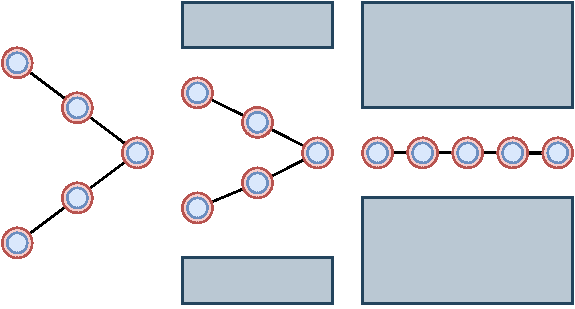
\includegraphics[width=0.6\textwidth]{paper1/images/idea.pdf}
    \caption{The self-reconfigurable V-shape formation can adjust its shape and navigate through narrow passages.}
    \label{fig:idea}
\end{figure}

Recently, advancements in path planning and obstacle avoidance techniques have contributed to the development of self-reconfigurable formation control algorithms. In \cite{8843165}, the angle-encoded particle swarm optimization algorithm is developed for the formation of multiple UAVs used in vision-based inspection of infrastructure. By incorporating constraints related to flight safety and visual inspection, the path and formation can be combined to provide trajectory and velocity profiles for each UAV. The work in \cite{FENG2022} developed a novel optimization method for multi-UAV formation to achieve rapid and accurate reconfiguration under random attacks. In \cite{Gao2022}, multi-UAV reconfiguration problems are modeled as an optimal problem with task assignment and control optimization. However, the focus of their work was on maintaining a fixed formation shape rather than self-reconfiguration in the presence of obstacles.

% \hl{Formation control in environments with obstacles and narrow passages presents challenges in obstacle avoidance, passing through constrained spaces, and so on \cite{Huang2019,Saska2020}. To address these challenges, building a self-reconfiguration formation control strategy is crucial. Such a strategy ensures robustness, adaptability, and efficient navigation, allowing the formation to autonomously adjust its shape to navigate through narrow gaps and avoid obstacles without external intervention. It enhances safety, and mission continuity, making autonomous multi-agent systems more capable and effective in complex and dynamic environments for various applications. Although research efforts have been made in the area of self-reconfigurable formation control, limited work has specifically addressed the challenges of self-reconfigurable formations in large obstacles and narrow environments. }

In this work, we propose a self-reconfigurable V-shape formation control algorithm for multiple UAVs operating in narrow space where the formation cannot maintain its initial shape when moving through this space. The algorithm allows the UAVs to form, maintain and reconfigure the desired V-shape formation by expanding/shrinking its two V-wings to avoid collisions with obstacles and maintain distances among the UAVs. According to the proposed design of distributed behaviors, the V-shape formations can open/close wings or merge into a straight line. Based on it, the UAVs can navigate through narrow passages, bypass obstacles, and optimize their trajectory in accordance to environmental conditions. The main contributions of our work are twofold: (i) develop a self-reconfiguration strategy that can adjust its shape in narrow space environments; and (ii) propose reconfiguration behaviors that navigate UAVs and maintain their shape.

% The remaining sections of this chapter are structured as follows. Section \ref{sec:0design} describes the design of the V-shape formation. Section \ref{sec:0control} presents our implementation of the behavior-based controller. Section \ref{sec:0result} shows simulation results. Our paper ends with conclusions drawn in Section \ref{sec:0conclusion}.
\section{V-Shape Formation Design} \label{sec:0design}
The V-shape formation is chosen due to its advantages in improving maneuverability and enhancing visibility for UAVs. Its modeling and design principles are presented as follows. 
\subsection{UAV model}
\begin{figure}
    \centering
    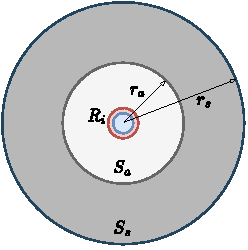
\includegraphics[width=0.3\textwidth]{paper1/images/model.pdf}
    \caption{The sensing range $r_s$ and alert range $r_a$ ($r_a<r_s$) of a UAV $R_i$}
    \label{fig:chap2_model}
\end{figure}
 
The formation consists of $n$ identical UAVs, each equipped with sensory modules for positioning and navigation such as Lidar, GPS and inertial measurement unit (IMU). The UAV is also equipped with a communication module that allows peer-to-peer communication among the UAVs. At height $h$, a UAV $R_i$ is modeled as a particle moving in a 2D plane located at that height with position $\mathbf{p}_i$ and heading angle $\psi_i$. The single-integrator kinematic model of UAV $R_i$ can be expressed as follows:
\begin{equation}
    \dot{\mathbf{p}}_i = \mathbf{v}_i,
\end{equation}
where $\mathbf{v}_i=[v_{ix},v_{iy}]^T$ is the velocity vector of UAV $R_i$. The heading angle $\psi_i$ then can be obtained as:
\begin{equation}
    \psi_i=\text{atan2}(u_{iy},u_{ix}).
\end{equation}

The communication range of each UAV $R_i$ is divided into two areas including the sensing area $S_s$ with radius $r_s$ and the alert area $S_a$ with radius $r_a<r_s$ so that $S_a\subset S_s$, as illustrated in Figure \ref{fig:chap2_model}.

\subsection{V-shape formation}
\begin{figure}
    \centering
    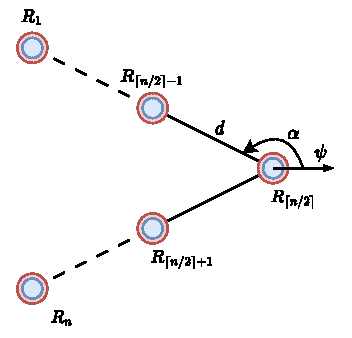
\includegraphics[width=0.4\textwidth]{paper1/images/v-shape.pdf}
    \caption{Illustration of the V-shape formation}
    \label{fig:chap2_vshape}
\end{figure}
In this work, the V-shape formation is constructed by two wings \cite{Dang2019}, as shown in Figure \ref{fig:chap2_vshape}. The wings are described by the desired distances between consecutive UAVs, $d$, and the bearing angle between the formation heading and each wing, $\alpha$. Without loss of generality, choose UAV $R_l$, with $l=\left\lceil{n}/{2}\right\rceil$, as the leader UAV located at the forefront of the formation. The desired distance $d_i$ and angle $\alpha_i$ between UAV $R_i$, $i\neq l$, and UAV $R_l$ are determined as follows:
\begin{equation}
\begin{aligned}
    d_i&=d\left\vert l-i\right\vert,\\
    \alpha_{i}&=\left\{ \begin{array}{cc}
\psi_{l}+\alpha & \text{if }i<l\\
\psi_{l}-\alpha & \text{if }i>l
\end{array}\right.
\end{aligned}
\label{eqn:chap2_desired}
\end{equation}

Thus, the desired position of UAV $R_i$ can be obtained as follows:
\begin{equation}
    \mathbf{p}_i^d=\mathbf{p}_l+d_i\left[\begin{array}{c}
\cos\alpha_{i}\\
\sin\alpha_{i}
\end{array}\right].
\label{eqn:chap2_desired_pose}
\end{equation}
\section{Distributed Formation Control Strategy} \label{sec:0control}
The formation control strategy aims to form, maintain and self-reconfigurate the V-shape formation in response to obstacles and narrow passages during UAV navigation. This adaptation is achieved through either expanding/shrinking two wings of the V-shape. It allows the UAV formation to navigate safely within confined spaces without encountering collisions. The proposed algorithm operates based on the use of distributed behavior-based control and artificial potential field approaches so that individual UAVs can make decisions and adjust the formation shape as needed. The strategy consists of two parts: maintaining formation and reconfigurating formation.

\begin{figure*}
    \centering
    \begin{subfigure}[b]{0.32\textwidth}
    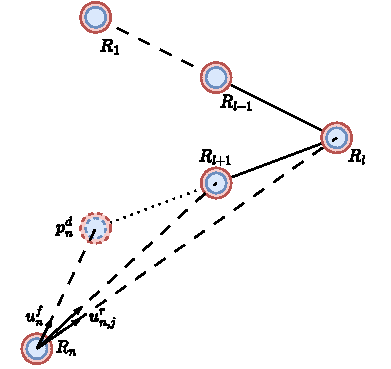
\includegraphics[width=\textwidth]{paper1/images/reconfiguration0.pdf}
    \caption{Disruption in formation}
    \label{fig:chap2_reconfig0}
    \end{subfigure}
    \begin{subfigure}[b]{0.32\textwidth}
    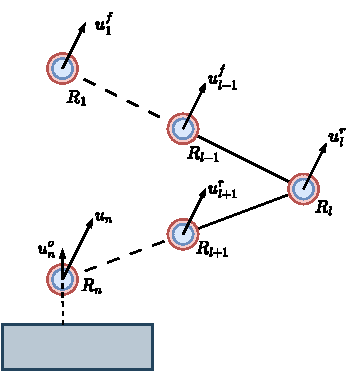
\includegraphics[width=\textwidth]{paper1/images/reconfiguration1.pdf}
    \caption{Obstacles from one side}
    \label{fig:chap2_reconfig1}
    \end{subfigure}
    \begin{subfigure}[b]{0.32\textwidth}
    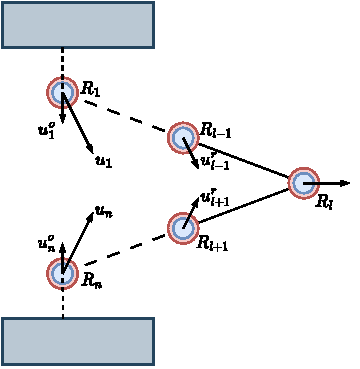
\includegraphics[width=\textwidth]{paper1/images/reconfiguration2.pdf}
    \caption{Obstacles from both sides}
    \label{fig:chap2_reconfig2}
    \end{subfigure}
    \caption{Self-reconfiguration of the V-shape formation based on the mechanism of pliers or scissors}
    \label{fig:chap2_reconfiguration}
\end{figure*}

\subsection{Formation maintenance strategy}
Behavior-based control is the approach that combines a set of distributed control modules, called behaviors, to achieve the desired objective \cite{Mataric2008, 736776}. In this work, the UAV formation is maintained based on the combination of the following behaviors.
\subsubsection{Formation behavior}
The formation behavior aims to guide UAVs to achieve their desired positions within the predefined formation. According to \eqref{eqn:chap2_desired_pose}, the desired position $\mathbf{p}_i^d$ of UAV $R_i$ in the formation can be obtained. Inspired by \cite{Dang2019,MirzaeeKahagh2020}, we define the formation behavior as follows:
\begin{equation}
    \mathbf{v}_i^f=-k_f\left(\mathbf{p}_i- \mathbf{p}_i^d\right) + \mathbf{v}_l,
    \label{eqn:chap2_uf}
\end{equation}
where $k_f>0$ is a positive formation gain. 

\subsubsection{Goal reaching behavior}
This behavior navigates the formation towards the desired location. To accomplish this objective, a target-tracking controller is formulated based on the relative position between the leader UAV and the goal. Let $\mathbf{p}_g$ be the goal position that the formation needs to reach. The goal reaching behavior is constructed as follows: 
\begin{equation}
    \mathbf{v}_i^g=-k_g\left(\mathbf{p}_i - \mathbf{p}_g\right),
    \label{eqn:chap2_ug}
\end{equation}
where $k_g>0$ is a positive tracking gain.

\subsubsection{Obstacle avoidance behavior}
During operation, the formation must avoid obstacles present in the environment. Let $\mathbf{p}_{io_h}$ be the closest point on the boundary of obstacle $o_h$ within the sensing range of UAV $R_i$. When that UAV senses obstacle $o_h$, it will create a thrust to maneuver and avoid the obstacle. The thrust is directed as follows:
\begin{equation}
    \mathbf{v}_{ih}^{o}=\left\{ \begin{array}{cc}
-k_o\left(\dfrac{1}{d_{io_h}^2} - \dfrac{1}{r_s^2}\right)\dfrac{\mathbf{p}_i-\mathbf{p}_{io_h}}{\left\Vert \mathbf{p}_i-\mathbf{p}_{io_h}\right\Vert}, & \text{if } d_{io_h} < r_s\\
0. & \text{otherwise}\\
\end{array}\right.
\end{equation}
where $k_o>0$ is a positive gain; $d_{io_h}$ is the distance between UAV $R_i$ and obstacle $o_h$. When considering all obstacles, the obstacle avoidance behavior of UAV $R_i$ are obtained as follows:
\begin{equation}
    \mathbf{v}_i^o=\sum_{h=1}^m{\mathbf{v}_{ih}},
    \label{eqn:chap2_uo}
\end{equation}
where $m$ is number of observable obstacles within the sensing range of UAV $R_i$.

\subsubsection{Collision avoidance behavior}
Apart from avoiding obstacles, the control algorithm also needs to adjust the UAV positions to avoid collision among them. To address this, we propose that UAVs $R_i$ and $R_j$ that are not in the same wing but within each other's sensing area, i.e., $\left\Vert \mathbf{p}_{ij}\right\Vert < r_{s}$, will exert a repulsive force to preventing the UAVs from entering the alert area $S_a$. Let $\mathbf{p}_{ij}=\mathbf{p}_i-\mathbf{p}_j$. The collision avoidance behavior is determined as follows:
\begin{equation}
    \mathbf{v}_{ij}^{c}=k_{c}\dfrac{e^{-\beta_{c}\left(\left\Vert \mathbf{p}_{ij}\right\Vert -r_{a}\right)}}{\left\Vert \mathbf{p}_{ij}\right\Vert -r_{a}}\dfrac{\mathbf{p}_i-\mathbf{p}_j}{\left\Vert \mathbf{p}_i-\mathbf{p}_j\right\Vert},
    \label{eqn:chap2_uc}
\end{equation}
where $k_c>0$ is a positive collision gain.

%The collision avoidance behavior of UAV in the same wing is further introduced in Section \ref{sec:0reconfig}.

\subsection{Self-reconfigurable formation strategy} 
\label{sec:0reconfig}
Inspired by the mechanics of pliers and scissors, which alter their shape through the application of opposing forces on their handle arms, the V-shape formation can open or close its wings based on the exertion of external forces. In our work, the force is produced based on the difference in the distances among the UAVs and their desired distances. Specifically, in case the formation encounters disruptions arising from improper positioning, as illustrated in Figure \ref{fig:chap2_reconfig0} where UAV $R_n$ deviates from the alignment, the combined force acts to guide it toward its desired location.

In the scenario depicted by Figure \ref{fig:chap2_reconfig1} where a force is exerted from one side, UAV $R_n$ responds by generating a thrust $\mathbf{v}_n^o$ to avoid a potential collision with obstacles thus resulting in the control signal $\mathbf{v}_n$. Accordingly, other UAVs on the same V-wing, including the leader UAV, also adjust their position based on the behavior control signal $\mathbf{v}_i^r$. As the leader UAV $R_l$ changes its position, the UAVs on the opposing wing realign themselves by formation behavior $\mathbf{v}_i^f$. As a result, the whole UAV formation tends to move towards the other side.

In another scenario, when obstacles impact the formation from both opposing sides, as depicted in Figure \ref{fig:chap2_reconfig2}, they affect UAVs $R_1$ and $R_n$, leading to the generation of obstacle avoidance behaviors denoted as $\mathbf{v}_1^o$ and $\mathbf{v}_n^o$. Other UAVs on the same wing respond by generating reconfiguration behaviors $\mathbf{v}_i^r$ that adjust the UAVs' position accordingly. As a result, the V-shape formation is able to shrink its wing to travel through narrow passages.

In our work, the aforementioned reconfiguration idea is implemented by the following equation:

\begin{equation}
    \mathbf{v}_{ij}^{r}=k_{r}\dfrac{\left|\left\Vert \mathbf{p}_{ij}\right\Vert -d_{ij}\right|^{\beta_r}}{\left(\left\Vert \mathbf{p}_{ij}\right\Vert -r_{a}\right)^{2}}\dfrac{\mathbf{p}_i-\mathbf{p}_j}{\left\Vert \mathbf{p}_i-\mathbf{p}_j\right\Vert},
    \label{eqn:chap2_ur}
\end{equation}
where $k_r>0$ is a positive reconfiguration gain, $\beta_r>0$ is the smoothness factor, $d_{ij}$ is the desired distance between two UAVs $R_i$ and $R_j$ n the same wing, $d_{ij}=d\left\vert i-j\right\vert$. In (\ref{eqn:chap2_ur}), the term $\left|\left\Vert \mathbf{p}_{ij}\right\Vert -d_{ij}\right|$ enables the UAVs to adjust their positions so that the desired distances among the UAVs are maintained. This behavior is also used as a collision avoidance behavior for the UAVs in the same wing.

\subsection{Overall strategy}
The overall distributed control strategy is obtained by combining the behaviors from all UAVs as follows:
\begin{equation}
    \mathbf{v}_{i}=\left\{ \begin{array}{cc}
\mathbf{v}_{i}^{g}+\mathbf{v}_{i}^{r}+\mathbf{v}_{i}^{c}+\mathbf{v}_{i}^{o}, & \text{if assigned as leader}\\
\mathbf{v}_{i}^{f}+\mathbf{v}_{i}^{r}+\mathbf{v}_{i}^{c}+\mathbf{v}_{i}^{o}. & \text{otherwise}
\end{array}\right.
\end{equation}

According to this function, the behaviors are automatically triggered in response to external influences or disturbances encountered by the formation. Once the desired state is achieved, the behavioral values are maintained resulting in stable operation of the UAV formation.
\section{Results and Discussion} \label{sec:0result}
In this section, we evaluate the performance of the proposed control strategy through different simulation scenarios.

\subsection{Simulation setup}
In the simulation, the UAV has the alert radius $r_a = 0.3$ m and the sensing radius $r_s = 2$ m. The control period is set at $0.02$ s. The maximum speed of each UAV is $2.0 \text{ m/s}$. The V-shape formation is defined with $d=0.8 \text{ m}$ and $\alpha=0.3\pi/4 \text{ rad}$. In our evaluation, 5 UAVs with V-shape formation are operated in the area of 46 m $\times$ 7 m with two large obstacles arranged to form a narrow passage as shown in Figure \ref{fig:chap2_result}.

\subsection{Results}
\begin{figure*}
    \centering
    \begin{subfigure}[b]{\textwidth}
        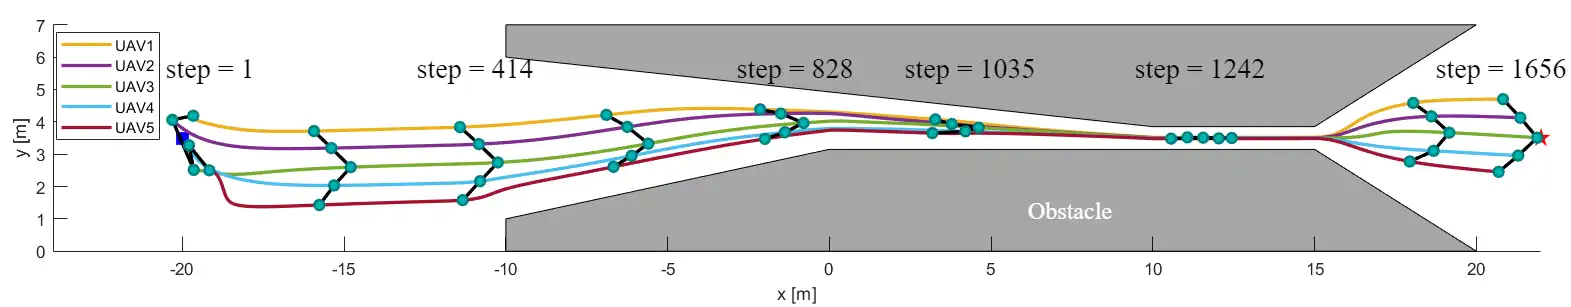
\includegraphics[width=\textwidth]{paper1/images/result.png}
        \caption{Trajectories of the UAVs in the formation}
        \label{fig:chap2_motion}
    \end{subfigure}
    \begin{subfigure}[b]{\textwidth}
        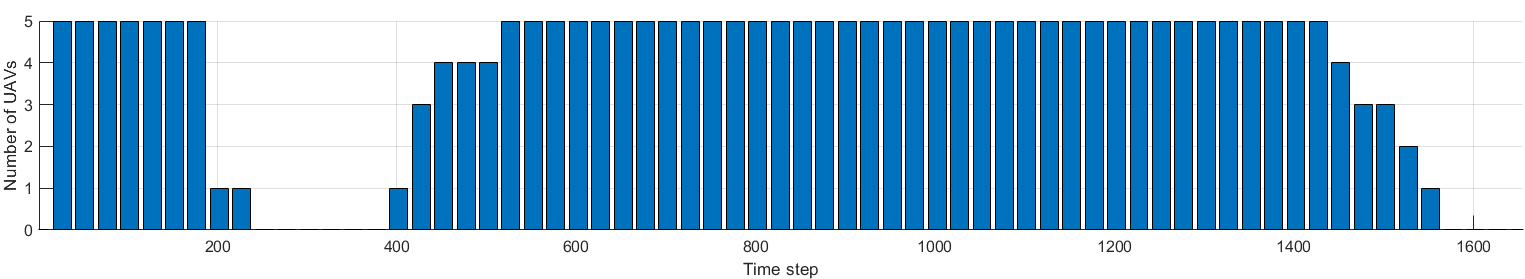
\includegraphics[width=\textwidth]{paper1/images/number.png}
        \caption{Number of UAVs activating reconfiguration behaviors over time}
        \label{fig:chap2_number}
    \end{subfigure}
    \caption{Simulation result of the V-shape formation moving through a narrow passage}
    \label{fig:chap2_result}
\end{figure*}

\begin{figure*}[t]
    \centering
    \begin{subfigure}[b]{0.49\textwidth}
    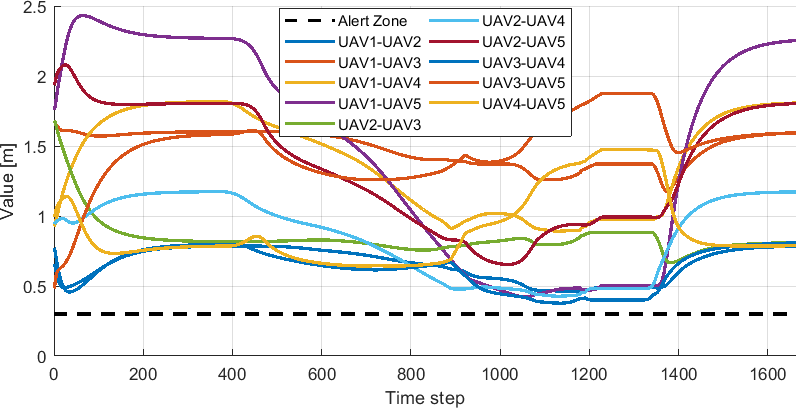
\includegraphics[width=\textwidth]{paper1/images/distance.png}
    \caption{Distances between each pair of UAVs over time}
    \label{fig:chap2_distance}
    \end{subfigure}
    \begin{subfigure}[b]{0.49\textwidth}
    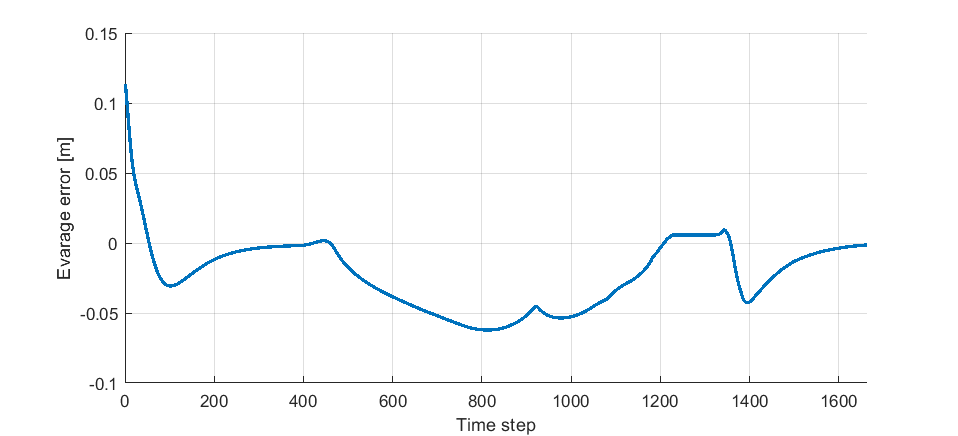
\includegraphics[width=\textwidth]{paper1/images/error.png}
    \caption{The average distance error of UAV formation}
    \label{fig:chap2_error}
    \end{subfigure}
    \begin{subfigure}[b]{0.49\textwidth}
    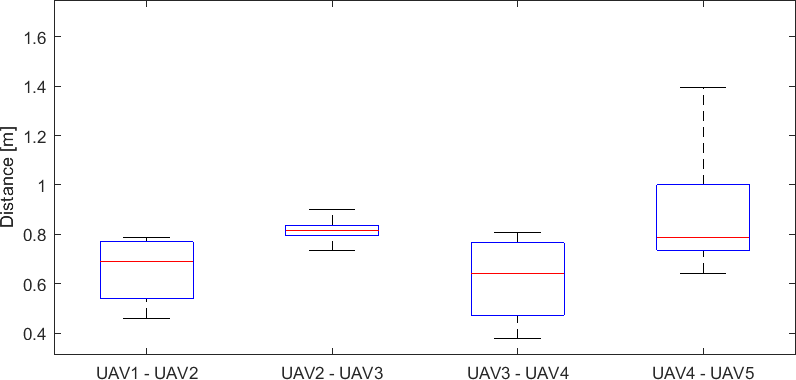
\includegraphics[width=\textwidth]{paper1/images/mean.png}
    \caption{The distance between consecutive UAVs}
    \label{fig:chap2_mean}
    \end{subfigure}
    \begin{subfigure}[b]{0.49\textwidth}
    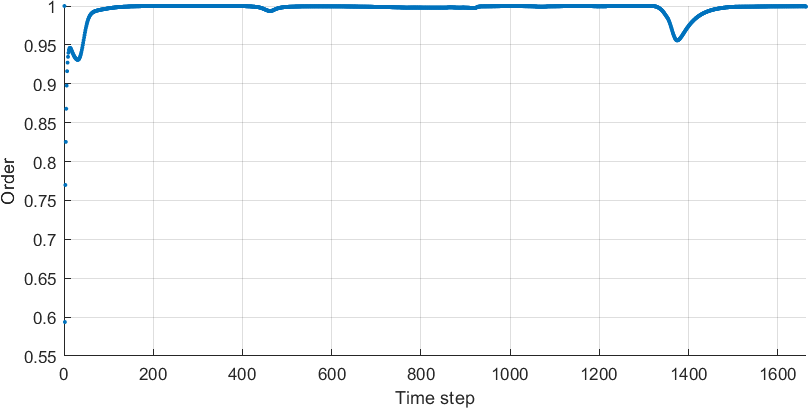
\includegraphics[width=\textwidth]{paper1/images/heading.png}
    \caption{Values of the \textit{order} metric $\Phi$ over time}
    \label{fig:chap2_heading}
    \end{subfigure}
    \caption{Evaluation of the proposed algorithm}
    \label{fig:chap2_eval}
\end{figure*}

\begin{table*}[!]
\centering
\caption{Statistical evaluation of the proposed strategy for several different scenarios}
\label{tbl:chap2_sta}
\begin{tabular}{C{1.2cm}C{1.5cm}C{1cm}C{1cm}C{2cm}C{2cm}C{3.5cm}}
\hline
Scenario & Number UAVs & $d$ & $\alpha$    & Average error (m) & Min distance (m) & Average distance of consecutive UAVs (m) \\ \hline
1     & 3        & 1.0   & $3\pi/4$             & 0.12333   & 0.48557   & 0.98788                      \\
2     & 5        & 1.0   & $3\pi/4$    & 0.12068   & 0.37383   & 0.96575                      \\
3     & 3        & 0.8   & $5\pi/6$    & 0.10942   & 0.48988   & 0.87599                      \\
4     & 3        & 1.0   & $4\pi/5$    & 0.13666   & 0.47581   & 1.0943                       \\
5     & 5        & 0.8   & $3\pi/4$    & 0.111     & 0.41279   & 0.88913     \\ \hline                
\end{tabular}
\end{table*}

Figure \ref{fig:chap2_result} shows the trajectories of the UAVs moving in the environment under the guidance of the proposed distributed controller. Initially, the UAVs are randomly positioned around a starting point (step 1). They then self-adjust to form the desired V-shape formation (step 414) based on the control signals generated by the formation and reconfiguration behaviors. As they encounter obstacles, the UAVs start to adjust their formation. This includes deforming the formation (steps 414-1035) and transitioning to a straight-line formation (step 1242) to navigate through narrow gaps. Upon successfully circumventing the obstacles, the UAVs readjust to form the desired V-shape and proceed toward the goal position (step 1656). The result can be verified in the simulation video shown in the footnote\footnote{Simulation video: {\fontfamily{qcr}\selectfont
\url{https://youtu.be/_6u7yMNOySc}}}. 

Figure \ref{fig:chap2_number} shows the number of UAVs activating their reconfiguration behavior over time. It can be seen that the UAVs activate this behavior when shaping the formation at the initialization stage, and during the process of adjusting their formation to adapt to the environment structure.

The statistical results of the evaluation of the proposed strategy are depicted in Figure \ref{fig:chap2_eval}. Figure \ref{fig:chap2_distance} shows the distances between the UAVs over time. It can be seen that those distances are all greater than the alert radius, which confirms the effectiveness of the control algorithm in avoiding collision among the UAVs.

Figure \ref{fig:chap2_error} presents the average distance error of the UAV formation over time. Initially, the error is large since the UAVs have not formed the desired shape. After the control algorithm realigns the UAV to their desired positions, the error quickly converges toward zero. While the formation navigates through the narrow passage, the error remains small, less than $0.06$ m. Figure \ref{fig:chap2_mean} shows the average distance between consecutive UAVs. It can be seen that the average distance fluctuates around the desired value for the V-shaped formation ($d=0.8$ m), which is desirable for the formation.

To further evaluate the performance of the proposed controller, an \textit{order} metric $\Phi$ that measures the similarity in the UAVs' direction is used \cite{Vicsek1995}. It takes the values in range $[0, 1]$ and is computed as follows:
\begin{equation}
    \Phi=\dfrac{1}{n}\left\Vert\sum_{i=1}^n{\left[\cos\psi_i, \sin\psi_i\right]^T}\right\Vert.
    \label{eq:order}
\end{equation}

According to (\ref{eq:order}), the order metric $\Phi$ is close to 1 when all UAVs have the same heading angle. Figure \ref{fig:chap2_heading} shows the value of $\Phi$ in our simulation. It can be seen that $\Phi$ is close to 1 during the movement of the formation, even when the formation avoids obstacles or traverses through a narrow passage. Changes in the heading angle increase when exiting the passage since the UAVs in the formation need to realign to the origin shape. However, the order metric then quickly converges to 1 when the UAVs form their desired formation. The results thus confirm the validity of the proposed control algorithm.

%\subsection{Discussion}
To further evaluate the performance of the proposed method, simulations on various scenarios such as narrow passages of varying widths and dense obstacle areas have been conducted. In addition, the number of UAVs and V-shape parameters, the desired distance, $d$, and the desired bearing angle, $\alpha$, are also varied. The results, including the average formation error, the closest distance between two UAVs, and the average distance between consecutive UAVs, are summarized in Table {\ref{tbl:chap2_sta}}. It is evident that the average formation error approximates $0.1m$, which is sufficient for the formation to maneuver in narrow spaces. Furthermore, the minimum distance between any pair of UAVs is larger than the collision threshold, $r_a$, and thus meets the requirement for collision avoidance. Finally, the average distance between consecutive UAVs closely aligns with the desired value, indicating the stability in the formation shape. These results confirm the validity and effectiveness of our proposed control strategy.
\section{Conclusion} \label{sec:0conclusion}
In this work, we have presented a new behavior-based controller to address the problem of UAV formation in narrow space environments. We developed several behaviors for each UAV and then proposed a function to combine them. Our approach allows the UAVs to form a V-shape formation with the capability to adjust their wings to avoid obstacles and travel through narrow passages. A number of simulation evaluations have been conducted and the results show that our control strategy is not only able to navigate the UAVs to form the desired V-shape formation but also provide them with the capability to reconfigure themselves to circumvent obstacles, avoid collisions, and traverse narrow passages in complex environments.


\chapter{Event-based Reconfiguration Control for Time-varying Robot Formation in Narrow Spaces}\label{paper2}

\noindent{\normalsize Published in:\\
\textit{Preprint}, 2024\\
% DOI:
Code: {\tt\url{https://github.com/duynamrcv/erc}}\\
Video: {\tt\url{https://youtu.be/rCIjgSqiWXg}}
}
\vspace{1cm}

\noindent\textit{\textbf{Abstract}}
Formation control plays a key role in coordinating multi-robot systems, especially in confined space environments where the risk of collisions is increased due to limited space. In this paper, we propose an event-based reconfiguration control (ERC) based on an artificial potential field that enhances the safety of time-varying robot formation (TVF) in a confined space. The proposed strategy includes two primary modes, \textit{``Formation''} and \textit{``Taigating''}, and provides flexible reconfiguration between original configuration and the straight-line configuration based on environmental perception. The proposed approach ensures that multi-robot systems maintain their desired configuration and collision-free trajectory. When a confined space is found to be insufficient to maintain the original formation, the configuration is either scaled down or transformed into a straight-line topology to maintain collision-free motion. A number of simulations, comparisons, and evaluations based on several metrics have been conducted to confirm the validity and superiority of the proposed approach.

\noindent\textbf{\textit{Keywords:}}
multi-robot system, time-varying formation, reconfiguration control, obstacle avoidance, event-triggering, artificial potential fields
% \end{keywords}

\section{Introduction}

With advancements in networked multi-agent technology, multi-robot systems (MRSs) have rapidly developed towards autonomy, offering various applications from warehouse automation to search and rescue operations~\cite {6303906,1335496}. A core element of these systems is a formation controller that enables the robots to collaborate in a desired configuration~\cite{1545539,Oh2015}. In rigid formation control, achieving the desired configuration involves setting a specific target distance for each swarm agent. However, with the increasing complexity of formation tasks, the formation configuration needs to be adjustable to meet specific task requirements. Time-varying formation (TVF) control thus has become essential for swarm robots~\cite{Dong2015,Dong2016}.

\begin{figure}
\centering
\begin{subfigure}[b]{0.4\textwidth}
    
    \centering
    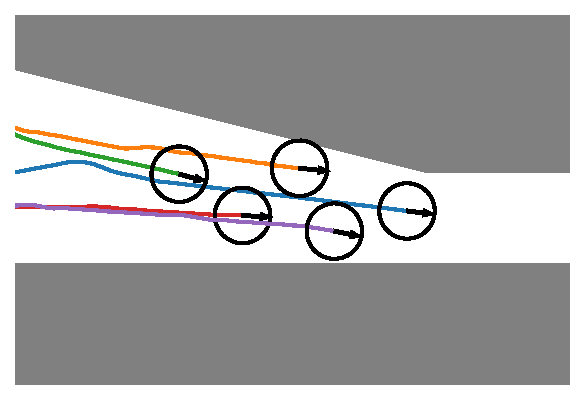
\includegraphics[width=\linewidth]{paper2/images/sample_bc.pdf}
    \caption{Pure formation control}
    \label{fig:1sample_bc}
\end{subfigure}
\begin{subfigure}[b]{0.4\textwidth}
    \centering
    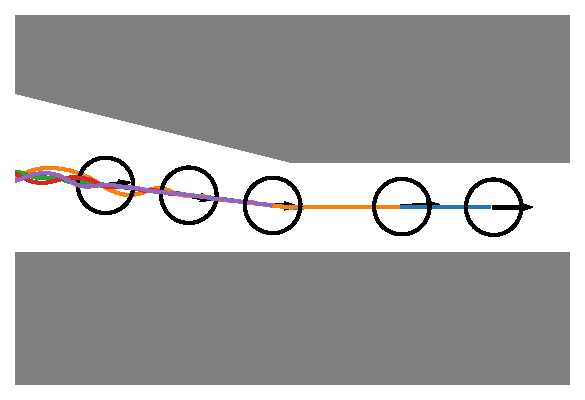
\includegraphics[width=\linewidth]{paper2/images/sample_edc.pdf}
    \caption{Proposed approach}
    \label{fig:1sample_edc}
\end{subfigure}
\caption{We develop an event-based reconfiguration control (ERC) method to guide a TVF through narrow spaces. \textit{Left:} Motion path of the TVF using purely behavior-based formation control~\cite{736776, Vsrhelyi2018}, which is collision with surrounding obstacles. \textit{Right:} Motion path of the TVF using our proposed approach, which safely navigates through the narrow spaces.}
\label{fig:1sample}
\end{figure}

Studies in~\cite{736776,Reynolds1987,Antonelli2009} show that biological swarm motion can be characterized by three primary behavioral rules: (i) \textit{cohesion}, which drives an agent toward to its neighbors; (ii) \textit{repulsion}, which pushes an agent away from its neighbors to prevent collisions; and (iii) \textit{alignment}, which aligns an agent to the dominant heading of its neighbors. For goal-oriented swarm motion, \textit{alignment} can be replaced by a \textit{migration} behavior so that each agent is directed in a desired orientation and moves at a preferred speed~\cite{6095129}. In complex environments, a fourth behavior called \textit{collision avoidance} can be added to guide the agent around obstacles~\cite{9565893, 9990164,1605401,10417519}. These behavioral rules are typically integrated into multi-robot systems through virtual forces within the artificial potential field (APF) to achieve coordinated movements~\cite{9981858,9561902,9990164}. Specifically, the APF has been used in~\cite{10417519,8716301,9565893} to navigate robot swarms through different environments, from open spaces to environments containing concave obstacles. In~\cite{9565893}, a fuzzy controller is added to allow the robot swarm to avoid complex obstacles while maintaining swarm connectivity. In~\cite{Vsrhelyi2018}, evolutionary optimization is combined with a behavioral model to enable stable and decentralized navigation for large-scale aerial robot swarms in confined spaces. However, using a fixed set of behaviors limits the flexibility of the swarm formation in response to abrupt changes in the environment, especially in spaces such as caves, corridors, and tunnels, and hence increases the risk of collisions~\cite{Saska2020,AlonsoMora2017}.

Apart from the behavior-based approach, studies in formation control can be further grouped into two primary categories: \textit{rigid formation}~\cite{Saska2020,Gmez2013,Roy2018,Ebel2017} and \textit{adaptive formation}~\cite{Fu2020,8843165,AlonsoMora2017,AlonsoMora2018}. In \textit{rigid formation}, the swarm can shrink or expand in size while preserving its overall shape. In~\cite{Saska2020}, a model predictive control is employed for rigid formation in which optimal control signals are generated for each robot in the swarm based on a shared map. In~\cite{Roy2018}, a region-based hierarchical control method is introduced for obstacle avoidance in confined spaces. The controller drives the robots to move cohesively within a virtual circular region that can contract to navigate around obstacles. A comprehensive control scheme is presented in~\cite{Ebel2017} for omnidirectional mobile robots to transport a plate through unknown environments collaboratively. The scheme uses graph-based path planning for obstacle avoidance and distributed model predictive control for optimal motion. Although rigid formations work well in open-space environments, they become ineffective in narrow spaces where the width of the space and the size of the formation directly affect navigation success. This challenge becomes critical when contracting the formation increases the risk of collision among the robots, as illustrated in Figure~\ref{fig:1sample_bc}.

In \textit{adaptive formation}, the swarm can transform into different configurations in adaptation to environmental conditions. In~\cite{Fu2020}, a reconfiguration strategy is combined with behavioral control for swarm navigation in dynamic environments. The strategy uses an auction-based market approach to generate solutions for formation movement. In~\cite{8843165}, particle swarm optimization is used to generate trajectories for a swarm of unmanned aerial vehicles (UAVs) that can reconfigure its formation for obstacle avoidance and task accomplishment. However, this approach is centralized and requires considerable computational resources to maintain an optimal configuration in real time. A robust adaptive formation control algorithm is introduced in~\cite{Mung2019} for a group of UAVs. The controller can steer the vehicles to form and maintain different formation patterns for flexible navigation. Generally, the adaptive formation methods are effective in guiding robots through complex environments as they enable flexible reconfiguration in response to environmental changes. However, there remains a need for a distributed, partial communication solution that ensures safe, efficient formation navigation while adapting effectively to environmental change.

In this work, we propose an event-based reconfiguration controller (ERC) for safe and effective navigation of a decentralized TVF in narrow environments, as given in Figure~\ref{fig:1sample}. The robots are equipped with local sensors and communication modules to collect information about the environment and other robots in the formation. The main contributions of this study are threefold:
\begin{enumerate}
    \item Define a set of individual behaviors that meet the reconfiguration control requirements, including goal-directed motion, formation maintenance, tailgating, and collision avoidance behaviors. Each behavior is designed for convenience in implementation via an artificial potential field.
        \item Propose an event-based reconfiguration controller with two modes, \textit{``formation''} and \textit{``tailgating''} capable of adapting the formation shape in response to environmental changes. The stability of the proposed approach has been demonstrated via the Lyapunov theorem.
    \item Extensive simulations and comparisons have been conducted to evaluate the robustness, scalability, and effectiveness of the proposed controller. Software-in-the-loop tests have also been conducted to verify its practical applicability. The source code of the proposed controller is publicly available for further research and practical implementation.
\end{enumerate}

The remaining sections of this paper are organized as follows. Section~\ref{sec2} presents the formation model and formulation. Section~\ref{sec3} introduces the proposed event-based reconfiguration control method. Simulation, comparison, and software-in-the-loop experimental results are shown in Section~\ref{sec4}. The paper ends with conclusions drawn in Section~\ref{sec5}.
\section{Preliminaries}\label{sec2}
\subsection{Model of robots}
Consider a swarm $\mathcal{N}$ that contains $n$ robots labelled $i\in\left\{1,...,n\right\}$. We model the swarm as a directed sensing graph $\mathcal{G}=\left(\mathcal{V},\mathcal{E}\right)$, where vertex set $\mathcal{V} = \left\{1,..., n\right\}$ represents the robots, and edge set $\mathcal{E}\subseteq\mathcal{V}\times \mathcal{V}$ contains the pairs of robots $\left(i, j\right)\in\mathcal{E}$ for which robot $i$ can sense robot $j$. We denote $\mathcal{N}_i=\left\{j\in\mathcal{V}|\left(i,j\right)\in\mathcal{E}\right\}\subset\mathcal{V}$ as the set of $n_i$ neighbours of a robot $i$ in $\mathcal{G}$.

\begin{figure}
    \centering
    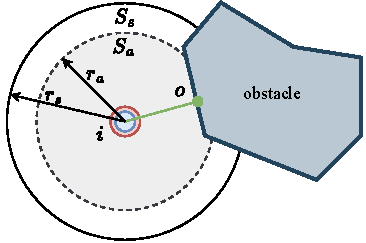
\includegraphics[width=0.45\textwidth]{paper2/images/model.pdf}
    \caption{Illustration of a robot with a local range sensor. Each robot is equipped with a local sensor with sensing area $S_s$ (solid while circle) being a circular disk within radius $r_s$. Additionally, alert area $S_a$ (dashed gray circle) is a circular disk within radius $r_a$, with $r_a\leq r_s$, which is the zone that robot will active the repulsive force to avoid collision. The set~$\mathcal{M}_i=\{o\}$ (green) is the nearest point from robot $i$ to obstacle.}
    \label{fig:1model}
\end{figure}

\begin{figure*}
    \centering
    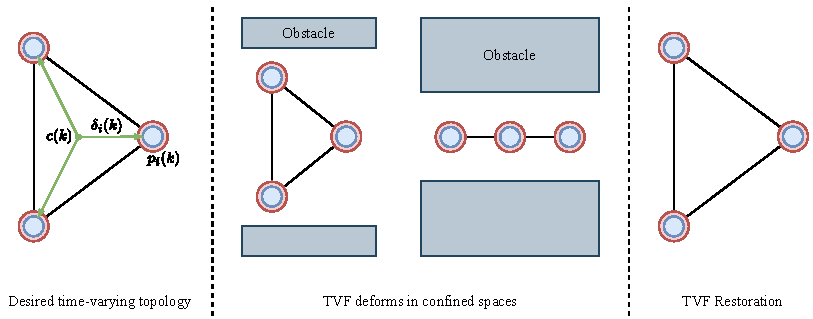
\includegraphics[width=0.9\textwidth]{paper2/images/problem.pdf}
    \caption{Schematic diagram of time-varying formation in the confined space}
    \label{fig:1problem}
\end{figure*}
In this study, the robots' dynamics are expressed in discrete time. The position, velocity, and control input of robot $i$ at time $t(k) = k\tau$ are denoted as $p_i(k), v_i(k), u_i(k) \in \mathbb{R}^3$, respectively, where $\tau$ represents the time step. The robots in the swarm are identical, each with a body radius $r$. Each robot $i$ is equipped with an inertial measurement unit (IMU) to determine its position and orientation in a desired direction, a range sensor, and a wireless ad-hoc network module for peer-to-peer communication with other robots. In this study, the communication delay between any two robots is assumed to be negligible~\cite{AlonsoMora2018,9527169}. Additionally, each robot is equipped with a circular sensor~\cite{8716301} that offers a $360^\circ$ field of view of the environment and can observed a maximum area $S_s$ within a radius $r_s$, as depicted in Fig.~\ref{fig:1model}. The set $\mathcal{M}_i(k) = \left\{o\right\}$ represents the observed obstacle points $o$ which is the nearest point on the obstacle's boundary at time $t(k)$. Additionally, a circular with the radius $r_a$ is denoted as an alert area that actives repulsive forces when robot $i$ sensing obstacles or its neighbors.

According to~\cite{Dong2015}, assuming that every robot in the swarm obeys a discrete linear system, given by
\begin{equation}
    x_i(k+1)=A_ix_i(k) + B_iu_i(k)
    \label{eqn:1model}
\end{equation}
where $A_i$ and $B_i$ are constant matrices. We consider the system to represent a robot with an underlying acceleration controller. The input $u_i$ is an acceleration command, and the state $x_i=\left[p_i,v_i\right]^T\in\mathbb{R}^6$ is a vector containing the position and velocity. The velocities and accelerations of the robots are bounded by constant vectors, i.e. $\left\Vert v_i(k)\right\Vert\leq v_\text{max}$ and $\left\Vert u_i(k)\right\Vert\leq u_\text{max}$.

\subsection{Problem formulation}

This paper addresses the safe formation control of time-varying formation (TVF) in confined space. The primary challenges addressed are:
\begin{enumerate}
    \item Ensuring collision-free navigation for the TVF, even when in the limited space environment.
        \item Incorporating an event-triggering mechanism into the TVF control, allowing the formation to deform to another safe configuration.
\end{enumerate}

Fig.~\ref{fig:1problem} provides the general schematic diagram of the research problem tackled in this study. Initially, the desired configuration assigned to the TVF is denoted $\delta_0$. At time $k$, the TVF can maintain the initial topology, i.e. $\delta(k)=\delta_0$. However, the confined space does not allow the formation maintaining topology $\delta_0$ due to the potential collision. As a result, a new topology is triggered to be applied depending on the surrounding space. Once the confined space is not detected by the robot, the initial topology $\delta_0$ of the formation is restored. With the proposed control approach, the formation configuration can be effectively managed. During the movement of the TVF, collaborative and collision avoidance controls are driven by the APF term in the proposed control strategy.

\begin{definition}\label{def_tvf}
(Time-Varying Formation~\cite{Dong2015,Dong2016} - TVF).  Let $\delta(k)=\left[\delta_1(k),...,\delta_n(k)\right]^T$ be a bounded time-varying vector that describes the desired formation configuration. The formation is said to achieve a TVF $\delta(k)$ if all robot $i$ in the formation satisfy:
\begin{equation}
    \lim_{k\to\infty}\sum_{i=1}^n\left\Vert p_i(k)-\delta_i(k)-c(k)\right\Vert=0,\quad\forall i\in\left\{1,...,n\right\}
\end{equation}
where $c(k)$ is called a formation center in the time $k$.
\end{definition}

\begin{definition}\label{def_pro}
(Safe Formation Control). Given the TVF as defined in Definition~\ref{def_tvf}, the safe formation control of TVF is said to be realized for any robot $i$ in the formation if the following conditions are simultaneously satisfied:
\begin{enumerate}
    \item Formation configuration
\begin{equation}
    \lim_{k\to\infty}\sum_{i=0}^n{\left\Vert\left(p_i(k)-\delta_i\right) - \left(p_j(k)-\delta_{j}\right)\right\Vert}=0
    \label{eqn:1form}
\end{equation}
for all $i,j\in\left\{1,...,n\right\}$, $i\neq j$.
%     \item Task completion
% \begin{equation}
%     \lim_{k\to T}\left\Vert\dfrac{1}{n}\sum_{i=1}^np_i-p_g\right\Vert=0
%     \label{eqn:1goal}
% \end{equation}
% where $T$ is a finite time, $p_g$ is the target position.
    \item Safe distance between robots
\begin{equation}
    \left\Vert p_i(k)-p_j(k)\right\Vert > 2r
    \label{eqn:1col}
\end{equation}
for all $i\in\left\{1,...,n\right\}$.
    \item Safe distance from obstacles
\begin{equation}
    \left\Vert p_i(k)-m\right\Vert > r
    \label{eqn:1obs}
\end{equation}
for all $i\in\left\{1,...,n\right\}$, and for all $m\in\mathcal{M}_i(k)$. 
\end{enumerate}
\end{definition}

\begin{remark}
According to the discrete linear model presented in~\eqref{eqn:1model}, this study primarily focuses on the changes in the position and velocity status of the robot. Based on Definition~\ref{def_tvf}, when~\eqref{eqn:1form} is established, robots reach the desired position, achieving the desired configuration. 
% Simultaneously, the velocity tends to zero once the tasks are completed~\eqref{eqn:1goal}. 
The establishment of \eqref{eqn:1col}~--~\eqref{eqn:1obs} ensure that the robot will not collide with obstacles or other robots in the formation, respectively.
\end{remark}

\subsection{Formation configurations}\label{sec:config}
Formation configurations are emerging while robots are cooperating and interacting with the confined space environments. In this study, we categorize formation configurations into two primary configurations:
\begin{enumerate}
    \item \textit{Original configuration:} This formation configuration is maintained if any surrounding space is large enough to maintain the originally defined configuration or to transform it by contraction. The configuration can be a V-shape, a polygon, or others.
        \item \textit{Straight line configuration:} This formation configuration is performed when the robot does not have enough space to maintain the original configuration, forcing it convert to this form for safety assurance~\cite{Fu2020}. This configuration is constructed by having a robot follow and keep desired distance from its leader.
\end{enumerate}
\section{Event-based Reconfiguration Control}\label{sec3}

To address the TVF problem, several potential force-based behaviors for each robot $i$ are used to synthetic to the proposed controller, which contains emergent strategies to navigate TVF to deal with the narrow space environment while ensuring the shape and the safety of TVF, named \textit{``formation''}, and \textit{``tailgating''}. In \textit{``formation''} mode, the TVF maintains the original configuration, while in \textit{``tailgating''} mode, the TVF transforms to the straight line configuration, as presented in Section~\ref{sec:config}. The detail of the proposed strategies is described in Figure~\ref{fig:1control_diagram}.

\begin{figure*}
    \centering
    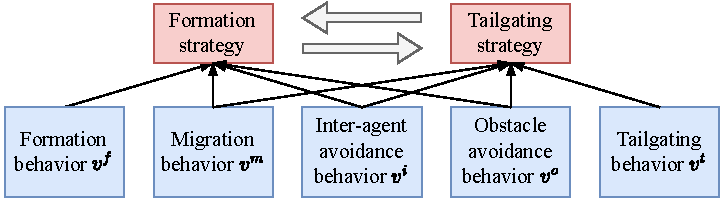
\includegraphics[width=0.85\textwidth]{paper2/images/control_diagram.pdf}
    \caption{Overview of the proposed event-based reconfiguration control. The proposed strategy is constructed by two primary emergent strategy, including \textit{``formation''} and \textit{``tailgating''}, which are highlighted by red boxes. There are five individual behaviors that contribute to the emergent strategy, which illustrated via blue boxes.}
    \label{fig:1control_diagram}
\end{figure*}

Our approach incorporates an event-triggering mechanism into the TVF that allows the swarm to adapt its formation shape in response to environmental conditions for safe navigation, as illustrated in Figure~\ref{fig:1problem}. Initially, the desired configuration assigned to the TVF is denoted $\mathbf{\delta}_0$. At time $k$, the TVF can maintain the initial topology, i.e. $\mathbf{\delta}(k)=\mathbf{\delta}_0$. However, the confined space does not allow the formation maintaining topology $\mathbf{\delta}_0$ due to the potential collision. As a result, a new topology is triggered to be applied depending on the surrounding space. Once the confined space is not detected by the robot, the initial topology $\mathbf{\delta}_0$ of the formation is restored. With the proposed control approach, the formation configuration can be effectively managed. During the movement of the TVF, collaborative and collision avoidance controls are driven by the APF term in the proposed control strategy.

\subsection{Individual behaviors}
According to~\cite{Vsrhelyi2018}, the potential field model is used to design individual behaviors a state-of-the-art model that allows robot swarm navigation in confined environments. From the original model, we design the rule of attraction for formation maintenance, tailgating and goal orientation; the rule of repulsion to prevent inter-robot collisions, and obstacle avoidance to avoid collisions with 
obstacles. 

Firstly, to ensure goal-directed motion in environments, a target reaching behavior is provided by a preferred velocity vector. We denote $v_\text{ref}$ is the preferred speed and $\mathbf{u}_\text{ref}$ is the preferred direction~\cite{6095129}. Then, the migration term, equal for every agent, corresponds to:
\begin{equation}
    \mathbf{v}_i^m=v_\text{ref}\mathbf{u}_\text{ref}
\end{equation}

Secondly, the formation behavior is designed as an attractive force that drive robots to move toward their desired positions. Denote $\kappa\in\mathbb{R}$ be the scale ratio, which can be determined in Section~\ref{sec:erc}. Thus, a relative position-based controller of the form to maintain the desired shape, and enhance the abilities of TVF with scalable capabilities, which is given as follow:
\begin{equation}
    \mathbf{v}^f_i=k_f\sum_{j=1}^n{\left(\mathbf{p}_j-\mathbf{p}_i-\kappa\left(\mathbf{\delta}_j-\mathbf{\delta}_i\right)\right)}
    \label{eqn:1uf}
\end{equation}
where $k_f>0$ is the formation control gain.

Next, the tailgating behavior is designed based on the relative position between each robot with other robot in the TVF, and used to navigate TVF pass through the narrow environment. Let robot $i$ follows robot ${l_i}$ within desired distance $d_\text{ref}$, with $d_\text{ref}>2r$,  an attractive force field for robot $i$ can be expressed as follows:
\begin{equation}
    \mathbf{v}_i^t=\begin{cases}
k_t\left(\mathbf{p}_{l_i}-\mathbf{p}_i-d_\text{ref}\dfrac{\mathbf{v}_{l_i}}{\left\Vert \mathbf{v}_{l_i}\right\Vert}\right)+\mathbf{v}_{l_i} & \text{if } l_i\neq-1\\
0 & \text{otherwise}
\end{cases}
    \label{eqn:1ut}
\end{equation}
where $k_t$ is the tailgating control gain. To determine the leader robot, the inner product $\tilde{\mathbf{p}}_{ij}$ of the difference between robot $j$ in the neighbor set $\mathcal{N}_i$ with robot $i$, $\mathbf{p}_j-\mathbf{p}_i$, and the desired direction, $\mathbf{u}_\text{ref}$, is given as follows:
\begin{equation}
    \tilde{\mathbf{p}}_{ij} = \left\langle (\mathbf{p}_j-\mathbf{p}_i),\mathbf{u}_\text{ref}\right\rangle
    \label{eqn:1tildep}
\end{equation}

As a result, the value of $\tilde{\mathbf{p}}_{ij}$ is positive, proving that robot $j$ is in front of robot $i$ according to $\mathbf{u}_\text{ref}$, and vice versa. For all robots $j$ in swarm, we obtain $\mathcal{P}_i=\left\{\tilde{\mathbf{p}}_{ij}\right\}$. The leader robot ${l_i}$ of robot $i$ is chosen as the closest robot in front of it, i.e.
\begin{equation}
     l_i=\begin{cases}
    \arg\min_{j}\left\{\tilde{\mathbf{p}}_{ij}\in\mathcal{P}_i\vert\tilde{\mathbf{p}}_{ij}\geq0\right\} & \exists~\tilde{\mathbf{p}}_{ij}\geq0\\ 
    -1 & \text{otherwise}
     \end{cases}
    \label{eqn:1li}
\end{equation}

Finally, inter-agent avoidance and obstacle avoidance behaviors are also designed to prevent collision. Denote $\mathcal{M}_i$ be the set of finite points on the obstacle's boundary, which are the closest to robot $i$, as illustrated in Figure~\ref{fig:1model}. Those repulsive forces are given as follows:
\begin{equation}
    \mathbf{v}_i^i=k_{i}\sum_{j=1,j\neq i}^n{\mathbf{v}_{ij}^i}
\end{equation}
\begin{equation}
    \mathbf{v}_i^o=k_o\sum_{\mathbf{o}\in\mathcal{M}}\mathbf{v}_{io}^o
\end{equation}
where $k_i,k_o>0$ is the inter-agent collision and obstacle avoidance gains, respectively. Denote $\mathbf{p}_{ij}=\mathbf{p}_i-\mathbf{p}_j$, and $\hat{\mathbf{p}}_{ij}=\dfrac{\mathbf{p}_{ij}}{\left\Vert \mathbf{p}_{ij}\right\Vert}$ be the relation position and the normalized vector between robot $i$ and robot $j$, respectively. Similarly, $\mathbf{p}_{io}$, and $\hat{\mathbf{p}}_{io}$ are the relative position and the normalized vector between robot $i$ and obstacle $\mathbf{o}$, respectively, with $\mathbf{o}\in\mathcal{M}_i$. Thus, the associated inter-agent avoidance $\mathbf{v}_{ij}^i$ and obstacle avoidance $\mathbf{v}_{io}^o$ are given as follows:
\begin{equation}
    \mathbf{v}_{ij}^{i}=\begin{cases}
    \dfrac{r_a-\left\Vert \mathbf{p}_{ij}\right\Vert}{r_a -2r}\hat{\mathbf{p}}_{ij} & \text{if }\left\Vert \mathbf{p}_{ij}\right\Vert<r_{a} \\
    0 & \text{otherwise}
    \end{cases}
    \label{eqn:1ui}
\end{equation}
\begin{equation}
    \mathbf{v}_{io}^{o}=\begin{cases}
    \dfrac{r_a-\left\Vert \mathbf{p}_{io}\right\Vert}{r_a -r}\hat{\mathbf{p}}_{io} & \text{if }\left\Vert \mathbf{p}_{io}\right\Vert<r_{a} \\
    0 & \text{otherwise}
    \end{cases}
    \label{eqn:1uo}
\end{equation}

\subsection{Event-based Reconfiguration Control strategy}\label{sec:erc}

As mentioned in Figure~\ref{fig:1control_diagram}, the proposed event-based reconfiguration control includes two emergent strategies to navigate TVF safely through narrow space environment while maintaining the shape and ensuring the safety of swarm. At each time step, each robot determine the mode itself based on the sensing data collected from local sensor. The overall strategy can be summarised as follows:
\begin{equation}
    \tilde{\mathbf{v}}_i=\begin{cases}
        \mathbf{v}_i^f+\mathbf{v}_i^m+\mathbf{v}_i^c+\mathbf{v}_i^o & \text{if mode = \textit{``formation''}}\\
        \mathbf{v}_i^t+\mathbf{v}_i^m+\mathbf{v}_i^c+\mathbf{v}_i^o & \text{if mode = \textit{``tailgating''}}
    \end{cases}
    \label{eqn:1v}
\end{equation}

To search the large parameter space $\Xi=\left\{k_f,k_t,k_i,k_o\right\}$ of the controller, evolutionary optimization can be used for highest-order flight and lowest number of collisions. The evaluation of the swarm behavior is based on a single fitness function that sums three independent values, including order, agent-safety, and obs-safety, smaller or equal to 1 (ideal case). The fitness is determined in simulations where the swarm is initialized with random positions in an environment where obstacles are  randomly placed. The description  to seek parameter values are similar and detailed in the~\cite{Vsrhelyi2018}.

To select the suitable mode at each time step, an event-based mode switching is designed to deal with the requirement to navigate a TVF through a narrow space environment. According to the individual behaviors and emergent strategies mentioned above, the mode of each robot can be changed based on its sense with environment around.

\begin{figure}
    \centering
    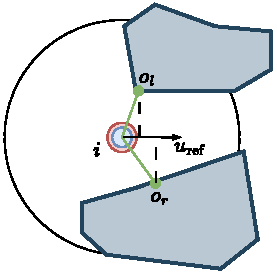
\includegraphics[width=0.35\textwidth]{paper2/images/we.pdf}
    \caption{Environment's width estimation}
    \label{fig:1we}
\end{figure}

Each obstacle point in the set $\mathcal{M}_{i}$ is clustered into two clusters on the left and right sides of the robot in $\mathbf{u}_\text{ref}$ direction. Denote $\mathbf{o}_l$ and $\mathbf{o}_r$ are the nearest obstacle points on the left and right sides, respectively, whose distance to the robot $i$ is minimum. If $\mathbf{o}_l$ and $\mathbf{o}_r$ exist, the width of the environment can be estimated by the magnitude of the cross product of the vector $(\mathbf{o}_r-\mathbf{o}_l)$ and the desired direction $\mathbf{u}_\text{ref}$ as follows:
\begin{equation}
    w_e= \left\Vert\left(\mathbf{o}_r-\mathbf{o}_l\right)\times \mathbf{u}_\text{ref}\right\Vert
    \label{eqn:1we}
\end{equation}

The estimation of the environment's width can be depicted in Figure~\ref{fig:1we}. Besides, the formation's width $w_f$ can be easily determined through the predefined formation topology. Given the widths of the environment and formation, the scaling factor $\kappa$, which contributes to \eqref{eqn:1uf}, can be computed as follows:
\begin{equation}
    \kappa = 
    \begin{cases} 
        \dfrac{w_e - 2r}{w_f} & \text{if } w_e \geq \lambda r \\
        0 & \text{otherwise}
    \end{cases}
    \label{eqn:1kappa}
\end{equation}

As a result, each robot $i$ can choose its mode and compute scaling factor $\kappa$. Denote $\lambda>2$ be the threshold to transform between two mode. As presented in Algorithm~\ref{alg:1our}, the desired velocity $\tilde{v}_i$ corresponding to its mode can be obtained.
\begin{algorithm}[h!]
\caption{Pseudocode of the ERC strategy}
\label{alg:1our}
Get a set of observed obstacle points $\mathcal{M}_i$\;
\If{$\mathcal{M}_i$ is empty}{
    mode $\leftarrow$ \textit{``formation''}\;
    $\kappa \leftarrow 1.0$\;
}
\Else{
    Determine the obstacle points $\mathbf{o}_l$, $\mathbf{o}_r$\;
    \If{$\nexists \mathbf{o}_l$ or $\nexists \mathbf{o}_r$}{
        mode $\leftarrow$ \textit{``formation''}\;
        $\kappa \leftarrow 1.0$\;
    }
    \Else{
        Get the space's width $w_e$\tcc*[r]{Eq. \ref{eqn:we}}
        \If{$w_e\leq\lambda r$}{
            mode $\leftarrow$ \textit{``tailgating''}\;
        }
        \Else{
            mode $\leftarrow$ \textit{``formation''}\;
            Estimate the desired formation width $w_f$\;
            \If{$w_e-2r\leq w_f$}{
                Compute the scaling factor $\kappa$\tcc*[r]{Eq. \ref{eqn:1kappa}}
            }
            \Else{
                $\kappa\leftarrow1.0$\;
            }
        }
    }
}
Compute desired velocity $\tilde{\mathbf{v}}_i$\tcc*[r]{Eq. \ref{eqn:1v}}
\Return $\tilde{\mathbf{v}}_i$\;
\end{algorithm}

After summing the contributions, we apply a cutoff on the acceleration at $u_\text{max}$ according to
\begin{equation}
    \mathbf{u}_i=\dfrac{\tilde{\mathbf{u}}_i}{\left\Vert\tilde{\mathbf{u}}_i\right\Vert}\min(\left\Vert\tilde{\mathbf{u}}_i\right\Vert, u_\text{max})
\end{equation}
where $\tilde{\mathbf{u}}_i(k+1) =(\tilde{\mathbf{v}}_i(k+1)-\tilde{\mathbf{v}}_i(k)) /\tau$. Then, we apply a cutoff on the speed at $v_\text{max}$, and get the velocity command $v_i$ as follows:
\begin{equation}
    \mathbf{v}_i=\dfrac{\tilde{\mathbf{v}}_i}{\left\Vert\tilde{\mathbf{v}}_i\right\Vert}\min(\left\Vert\tilde{\mathbf{v}}_i\right\Vert, v_\text{max})
\end{equation}

\subsection{Stability analysis}
\begin{theorem}\label{the:stability}
Given the TVF as described in~\eqref{eqn:1model}, under the control law given in \eqref{eqn:1v}, the TVF asymptotically converges to the desired configuration.
\end{theorem}
\begin{proof}
To prove Theorem~\ref{the:stability}, we consider the negligible effect of collision avoidance behaviors and also neglect the constant impact of migration behavior, for any time $t(k)$, thus we conduct a stability analysis of the TVF in main contributions, i.e. formation and tailgating behaviors, which located in two separate modes, \textit{``formation''} and \textit{``tailgating''}, as mentioned in Section~\ref{sec:config}, which together ultimately lead to our conclusion.

\textbf{Mode \textit{``formation''}:} Denote $L$ be the Laplacian matrix of the interaction topology graph of the swarm. Due to the fully connected, the entries of $\mathbf{L}=\left[l_{ij}\right]$ are given as follows:
\begin{equation}
    l_{ij}=\begin{cases}
    -1 & \text{if }i\neq j \\
    n-1 & \text{if }i=j
    \end{cases}
\end{equation}

The control law \eqref{eqn:1uf} can be shown as follows:
\begin{equation}
    k_f\sum_{j=1}^n{\left(\mathbf{p}_j-\mathbf{p}_i-\kappa \delta_{ji}\right)}=k_f\sum_{j=1}^n{\left(\mathbf{p}_j-\mathbf{p}_i\right)}+\mathbf{b}_i
\end{equation}
where the bias $\mathbf{b}_i=-k_f\sum_{j=1}^n\kappa \delta_{ji}$.  In order to use the properties of the Laplacian matrix, the dynamics of the swarm system with the control law can be expressed as follows:
\begin{equation}
    \dot{\mathbf{P}}=-k_f\mathbf{L}\mathbf{P}+\mathbf{B}
\end{equation}
where $\mathbf{P}=\left[\mathbf{p}_1,...,\mathbf{p}_n\right]^T$, $\mathbf{B}=\left[\mathbf{b}_1,...,\mathbf{b}_n\right]^T$ and $\mathbf{L}$ is the Laplacian matrix of the interaction topology graph of the formation. For these values of its elements the Laplacian matrix has only one zero eigenvalue and the rest of its eigenvalues are positive and the same. Note also that the vector $\mathbf{B}$ is an eigenvector of $\mathbf{L}$ with the corresponding eigenvalue $n$ and:
\begin{equation}
    \mathbf{L}\mathbf{B}=n\mathbf{B}
\end{equation}

Defined the Lyapunov-like function for the TVF system as follows:
\begin{equation}
    V_f=\dfrac{1}{2}\left(\mathbf{P}-\dfrac{1}{k_fn}\mathbf{B}\right)^T\left(\mathbf{P}-\dfrac{1}{k_fn}\mathbf{B}\right)
\end{equation}

Talking the first derivative of $V_f$ gives
\begin{equation}
\begin{aligned}
    \dot{V}_f&=\left(\mathbf{P}-\dfrac{1}{k_fn}\mathbf{B}\right)^T\left(-k_f\mathbf{L}\mathbf{P}+\mathbf{B}\right)\\
    &=-k_f\left(\mathbf{P}-\dfrac{1}{k_fn}\mathbf{B}\right)^T\mathbf{L}\left(\mathbf{P}-\dfrac{1}{k_fn}\mathbf{B}\right)\leq0
\end{aligned}
\end{equation}

According to the LaSalle’s invariance
principle, it can be stated that as $k\to\infty$ the state $\mathbf{P}$ will converge to the largest invariant subset $\Omega=\left\{\mathbf{P}|\dot{V}_f=0\right\}$. In other words, the formation will close to the desired shape.

\textbf{Mode \textit{``tailgating''}:} In case robot $i$ do not have it leader, we do not analysis the stability, because this robot do not contribute to the configuration maintenance of the TVF. Otherwise, in case robot $i$ has its leader $l_i$, we define a candidate Lyapunov function as follows:
\begin{equation}
    V_{t}=\dfrac{1}{2}\left(\mathbf{p}_{l_i}-\mathbf{p}_{i}-d_\text{ref}\dfrac{\mathbf{v}_{l_i}}{\left\Vert \mathbf{v}_{l_i}\right\Vert}\right)^{T}\left(\mathbf{p}_{l_i}-\mathbf{p}_{i}-d_\text{ref}\dfrac{\mathbf{v}_{l_i}}{\left\Vert \mathbf{v}_{l_i}\right\Vert}\right)
\end{equation}

Taking the first derivative of $V_t$, gives:
\begin{equation}
    \dot{V}_{t}=\left(\mathbf{p}_{l_i}-\mathbf{p}_{i}-d_\text{ref}\dfrac{\mathbf{v}_{l_i}}{\left\Vert \mathbf{v}_{l_i}\right\Vert}\right)^{T}\left(\mathbf{v}_{l_i}-\mathbf{v}_{i}\right)
\end{equation}

By using the control law $\mathbf{v}^t_i$ in \eqref{eqn:1ut}, $\dot{V}_t$ becomes:
\begin{equation}
    \dot{V}_{t}=-k_{t}\left(\mathbf{p}_{l_i}-\mathbf{p}_{i}-d_\text{ref}\dfrac{\mathbf{v}_{l_i}}{\left\Vert \mathbf{v}_{l_i}\right\Vert}\right)^{T}\left(\mathbf{p}_{l_i}-\mathbf{p}_{i}-d_\text{ref}\dfrac{\mathbf{v}_{l_i}}{\left\Vert \mathbf{v}_{l_i}\right\Vert}\right)\leq0
\end{equation}

Therefore, the Lyapunov stability is satisfied. That leads to robot $i$ converges to its leader $l_i$ and keep behind a distance $d_\text{ref}$ along its leader direction. As a result, the straight line configuration can be guaranteed.
\end{proof}

\begin{remark}
In the research of this chapter, decentralized control architecture is adopted for the TVF. Each robot in the formation can decide the mode itself based on information collected from the surrounding environment. The event-triggering condition designed in Algorithm~\ref{alg:1our} is also distributed and presented in the form of compact sets. Besides, the control law \eqref{eqn:1v} demonstrates stability based on Lyapunov theory. Under the action of the designed control law, the TVF will asymptotically achieve the desired configuration in both modes.
\end{remark}
\section{Results}\label{sec4}
\subsection{Simulation and Comparison}
\begin{figure*}[!h]
\begin{subfigure}[b]{\textwidth}
    
    \centering
    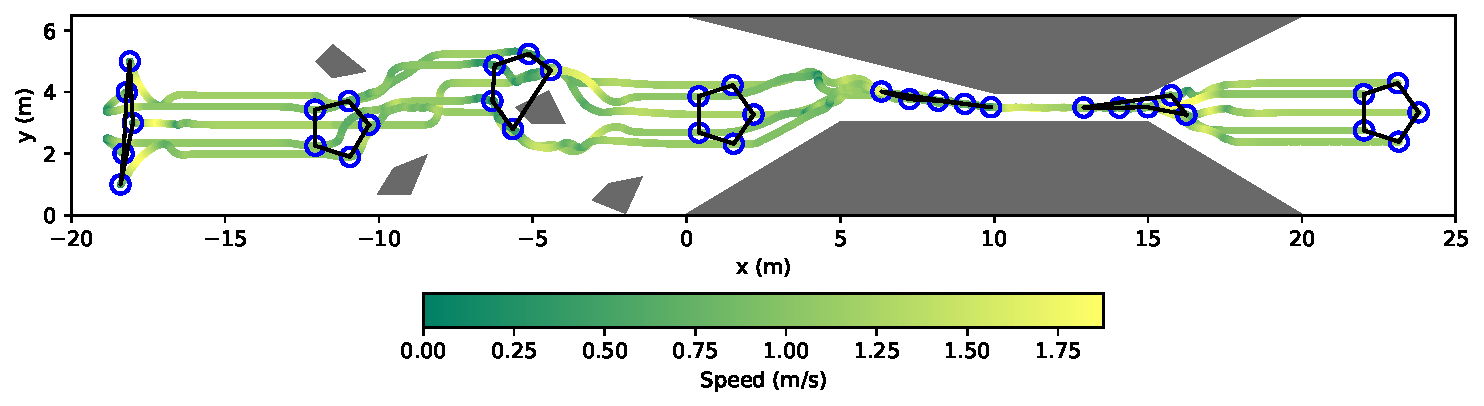
\includegraphics[width=0.9\textwidth]{paper2/images/path_edc_shape1.pdf}
    \caption{Pentagon configuration}
    \label{fig:1path_edc1}
\end{subfigure}
\begin{subfigure}[b]{\textwidth}
    \centering
    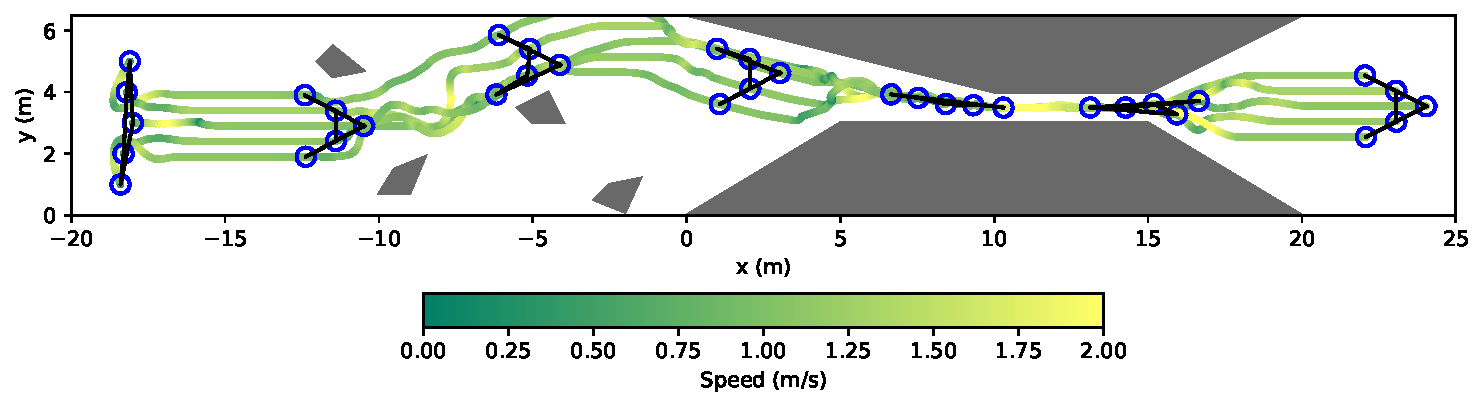
\includegraphics[width=0.9\textwidth]{paper2/images/path_edc_shape2.pdf}
    \caption{V-shape configuration}
    \label{fig:1path_edc2}
\end{subfigure}
\caption{Motion paths and velocity profiles of the proposed \textit{EFRC} strategy in multiple configurations.}
\label{fig:1path}
\end{figure*}

\begin{figure*}[!h]
\begin{subfigure}[b]{0.49\textwidth}
    
    \centering
    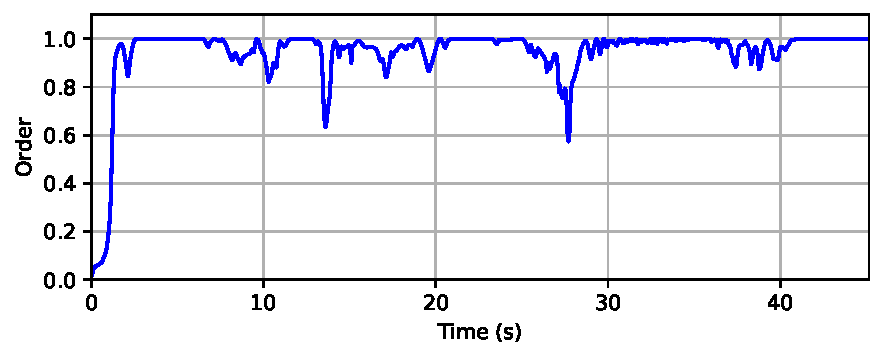
\includegraphics[width=\linewidth]{paper2/images/order_edc_shape1.pdf}
    \caption{Pentagon configuration}
    \label{fig:1order_edc1}
\end{subfigure}
\begin{subfigure}[b]{0.49\textwidth}
    \centering
    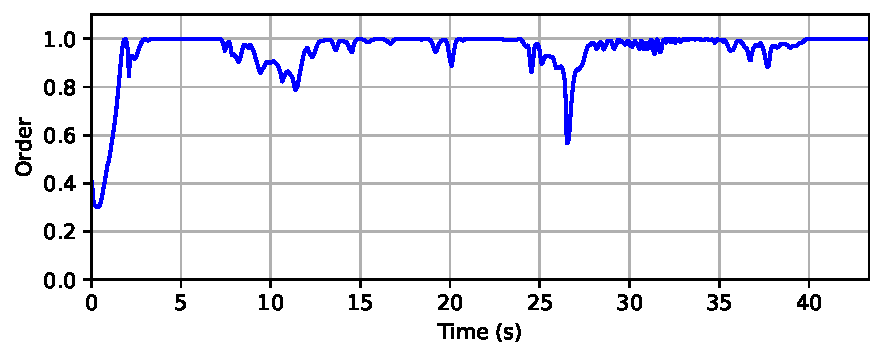
\includegraphics[width=\linewidth]{paper2/images/order_edc_shape2.pdf}
    \caption{V-shape configuration}
    \label{fig:1order_edc2}
\end{subfigure}
\caption{The \textit{order} values of the proposed \textit{EFRC} strategy}
\label{fig:1order}
\end{figure*}

\begin{figure*}[!h]
\begin{subfigure}[b]{0.49\textwidth}
    
    \centering
    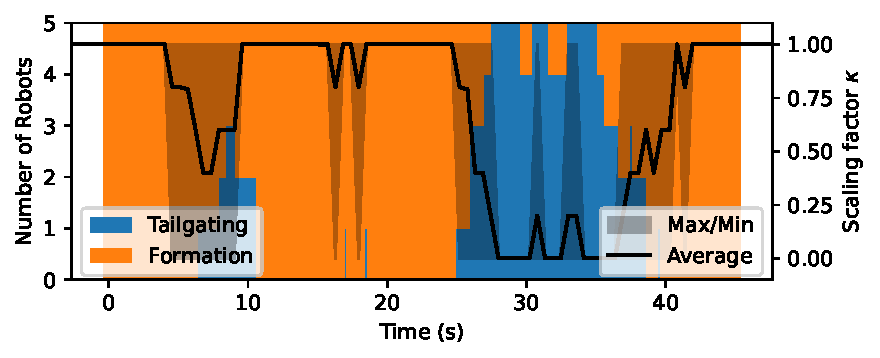
\includegraphics[width=\linewidth]{paper2/images/mode_edc_shape1.pdf}
    \caption{Pentagon configuration}
    \label{fig:1mode_edc1}
\end{subfigure}
\begin{subfigure}[b]{0.49\textwidth}
    \centering
    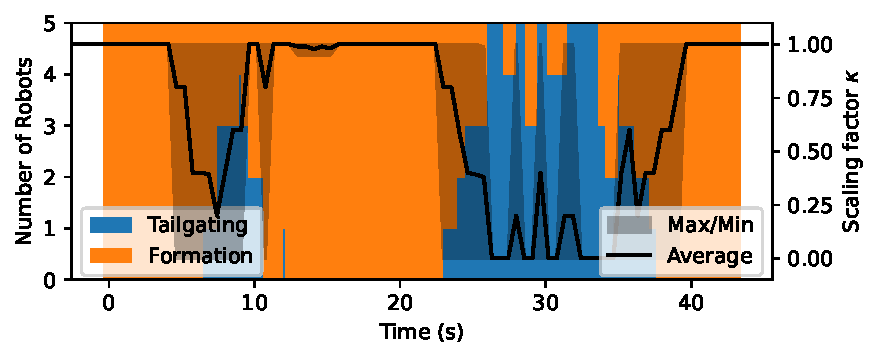
\includegraphics[width=\linewidth]{paper2/images/mode_edc_shape2.pdf}
    \caption{V-shape configuration}
    \label{fig:1mode_edc2}
\end{subfigure}
\caption{Correlation of number of robots and scaling factor of the proposed \textit{EFRC} strategy}
\label{fig:1mode}
\end{figure*}

% The simulations are run on AMD Ryzen 5 5500U with a base frequency of 2.1 GHz. 
The proposed strategy is tested in a complex environment, which consists of 2 areas of different obstacle types, one area is the forest-liked environment, whose obstacle densities is 0.05 obs/m$^2$ (for $-12$~m $<x<0$~m), another area is the width-varying cave-like environment with the most narrowed space is 1~m (for $0$~m $<x<20$~m). The TVF starts randomly from the left-hand side of the environment and has a mission to travel through the confined space to the right-hand side, with the desired direction $u_\text{ref}=\left[1,0,0\right]^T$. We set up a formation with 5 homogeneous robots with two formation configurations, including V-shape and polygon configurations, when the TVF transforms to \textit{``Tailgating''} mode, the desired distance for a robot to follow its leader is set by $d_\text{ref}=1$~m. They have constraints with $v_\text{max}=2$~m/s and $u_\text{max}=2$~m/s$^2$. The control period is set at $\tau=0.1$~s. The comparison is done with pure behavior-based control (\textit{BC})~\cite{736776,Vsrhelyi2018}. For comparison between the different methods, the following performance metrics are used: success rate, mean speed, and mean acceleration cost $(\sum{\left\Vert u(k)\right\Vert^2}/{nT})$, with $T$ is the total travel time of the TVF. The parameters used in both strategies are the same to ensure fairness.

In the simulation, we examined how the \textit{EFRC} guided a TVF to navigate through confined spaces. The motion paths and corresponding velocity profile are presented in Fig.~\ref{fig:1path}. Both two formations, including polygon and V-shape configurations, successfully navigate through confined spaces, which include forest-like and tunnel-like environments. Initially, all robots were on the left-hand side, which did not form the desired configuration. They move in the desired direction and form to the predefined shape. Whenever obstacles are detected, the robot activates the obstacle avoidance behavior, there is no narrow space in the first area, and robots in the formation maintain the \textit{``Formation''} mode. Once narrow space is observed, the TVF transforms to \textit{``Tailgating''} mode, which is assigned itself by each robot observation. The straight line configuration is then created, which can help the formation pass through the gap. When the robot escapes the narrow passage, the mode turns back to \textit{``Formation''} mode, which reforms to the desired configuration. Finally, the formation successfully passes through the confined space. Fig.~\ref{fig:1path} presents the motion paths of the TVF, which are conducted by the proposed strategy in multiple configurations.

To further investigate the effectiveness of the proposed strategy, the \textit{order} $\Phi$ metric is defined to measure the heading disturbance of robots in formation during movement. The order's values are in $\left[0,1\right]$, and if the formation has no heading, the order is close to 1 \cite{Vicsek1995}.
\begin{equation}
    \Phi=\dfrac{1}{n}\left\Vert\sum_{i=1}^n{\dfrac{v_i}{\left\Vert v_i\right\Vert}}\right\Vert
\end{equation}
where $v_i$ is the velocity of robot $i$.

Fig.~\ref{fig:1order} illustrates the order information of the TVF's heading throughout the movement process. The figures reveal that the heading order of the swarm in both two scenarios during movement is satisfactory ($\Phi = 1$), When the formation encounters obstacles, the \textit{order} value is changed but still forms the overall configuration. However, disorderliness in the heading order becomes apparent during the transition from \textit{``Formation''} to \textit{``Tailgating''} and vice versa. This is because the structure of the formation undergoes a significant change, resulting in a disorderly heading order.

Fig~\ref{fig:1mode} describes the correlation between the number of robots in different modes and the scaling factor $\kappa$ to evaluate the effectiveness of the synthesized controllers in the proposed deformation strategy. When the TVF encounters obstacles, the configuration is adapted based on the observation of each robot. As a result, the mode of each robot is different at the same time. Also, the scaling factor $\kappa$ is different between robots in the TVF, due to its position and the observation. In collision-free, all robots in the TVF remain in \textit{``Formation''} mode, which contributes to maintaining the original configuration. On the other hand, when narrow space is detected by all robots, the mode transforms to \textit{``Tailgating''}, which forces robots to the straight line configuration to safely navigate through narrow space. The value of $\kappa=0$ when all robots in the TVF are in the \textit{``Tailgating''} mode.

\begin{table}
\caption{Comparison between \textit{BC} and our method, \textit{EFRC} . Each comparison is over 10 simulations of 5 robots in two different configurations. The metrics displayed in the table are the success rate, mean speed, and mean acceleration cost.}
\label{tbl:com}
\centering
\begin{tabular}{C{3.2cm} C{2.cm} C{2.0cm} C{3.0cm} C{3.0cm}}
\hline\hline
Configuration             & Strategy & Succ. & Mean speed (m/s) & Mean Acc. cost (m$^2$/s$^4$)  \\ \hline
\multirow{2}{*}{Pentagon} & EFRC      & \textbf{10/10}        & 0.6773   & \textbf{3.6873}          \\
                          & BC       & 0/10    & \textbf{0.7785}   & 4.3874      
                          \\ \hline
\multirow{2}{*}{V-shape}  & EFRC      & \textbf{10/10}        & 0.7129   & \textbf{4.0978}          \\
                          & BC       & 0/10   & \textbf{0.8877}      & 4.9402 \\ \hline\hline    
\end{tabular}
\end{table}

To further verify the effectiveness of the proposed strategy against the pure behavioural-based control (\textit{BC})~\cite{736776,Vsrhelyi2018}, Table~\ref{tbl:com} presents a comparison between proposed strategy, \textit{EFRC} and \textit{BC}. It can be seen that the proposed \textit{EFRC} strategy outperforms the \textit{BC} in success rate, which can navigate formation passes through a confined space without any collision. Meanwhile, the \textit{BC} always fails when encountering a narrow space (see Fig.~\ref{fig:1sample}). The mean acceleration cost per time is also smaller than the \textit{BC}, because \textit{BC} costs more energy to deal with the surrounding obstacles. The \textit{EFRC} provides an effective method to deal with obstacles by the adaptation configuration. However, the mean speed of the TVF is slightly smaller than the standard approach, due to the translation mode while moving affect to the speed down of the TVF.

\subsection{Validation on the software-in-the-loop Gazebo}
\begin{figure*}[h!]
    \centering
    \begin{subfigure}[b]{0.45\textwidth}
    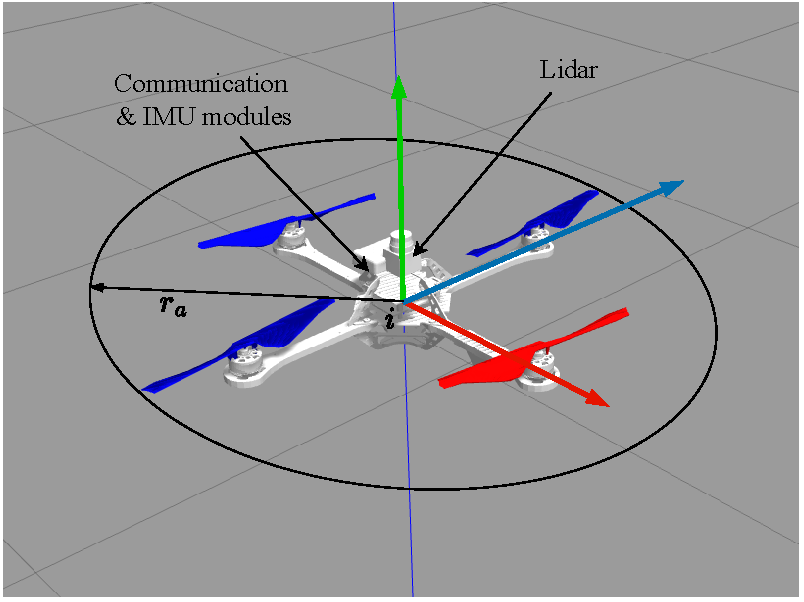
\includegraphics[width=\textwidth]{paper2/images/gazebo_uav.pdf}
    \caption{Gazebo SIL model}
    \label{fig:1gazebo_uav}
    \end{subfigure}
    \begin{subfigure}[b]{0.44\textwidth}
    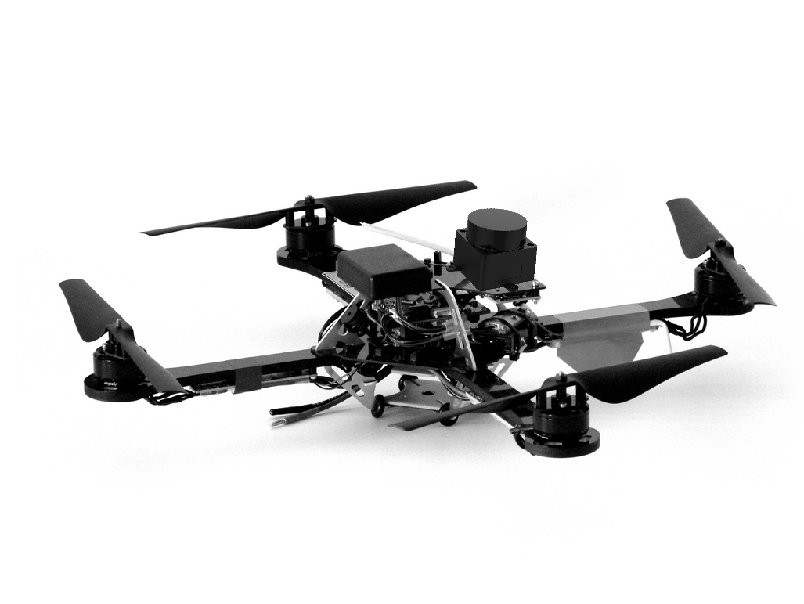
\includegraphics[width=\textwidth]{paper2/images/hummingbird.pdf}
    \caption{Real UAV model \cite{Furrer2016,Bui2022}}
    \label{fig:1gazebo_real}
    \end{subfigure}
    \caption{Used Hummingbird UAV model}
    \label{fig:1gazebo_setup}
\end{figure*}

\begin{figure*}[h!]
    \centering
    \begin{subfigure}[b]{0.495\textwidth}
    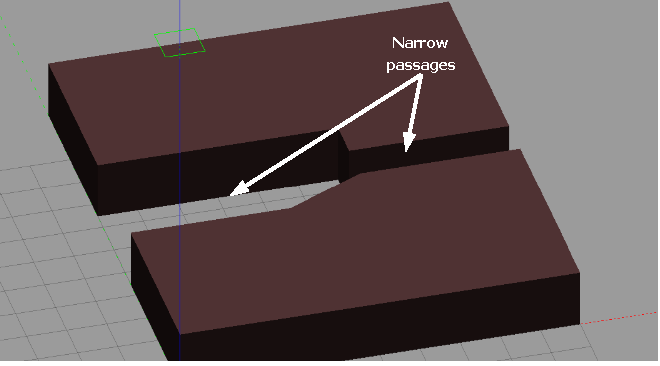
\includegraphics[width=\textwidth]{paper2/images/gazebo_env.pdf}
    \caption{The Gazebo environment}
    \end{subfigure}
    \begin{subfigure}[b]{0.40\textwidth}
    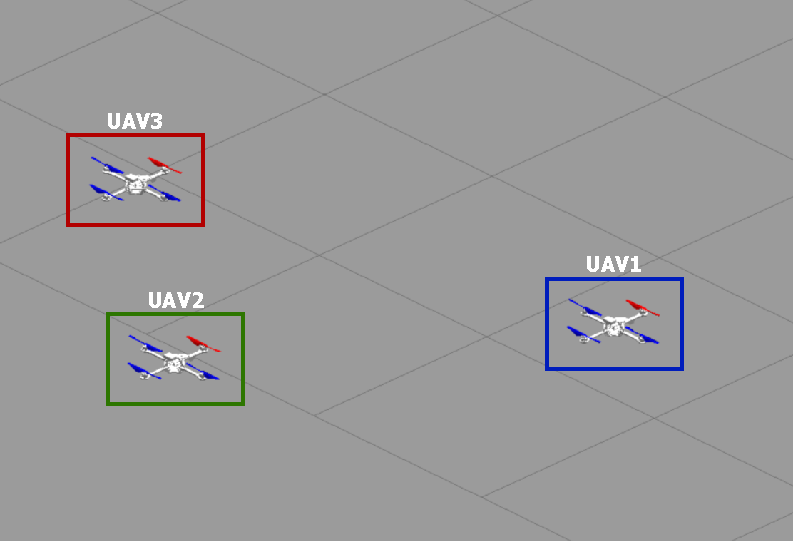
\includegraphics[width=\textwidth]{paper2/images/gazebo_init.pdf}
    \caption{Random initial positions}
    \label{fig:1gazebo_init}
    \end{subfigure}
    \caption{The environment in SIL test}
    \label{fig:1gazebo_env}
\end{figure*}

\begin{figure*}
    \centering
    \begin{subfigure}[b]{0.48\textwidth}
    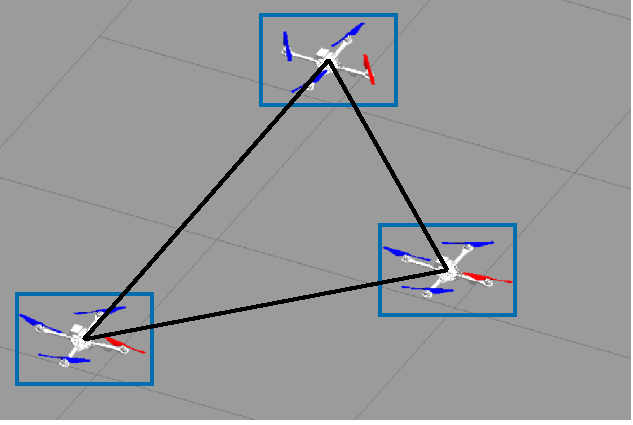
\includegraphics[width=\textwidth]{paper2/images/gazebo_res1.pdf}
    \caption{Maintain triangle formation from random}
    \label{fig:1gazebo_1}
    \end{subfigure}
    \begin{subfigure}[b]{0.48\textwidth}
    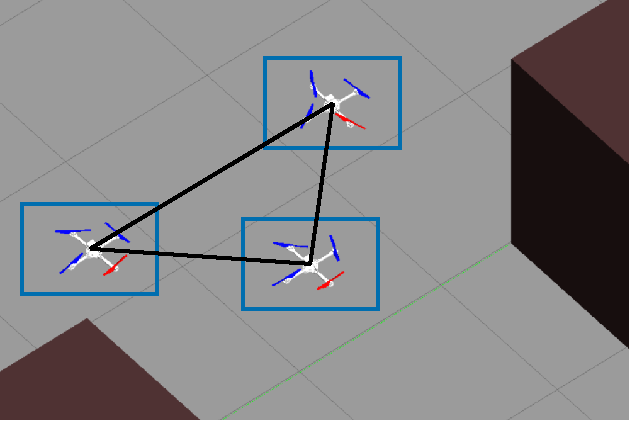
\includegraphics[width=\textwidth]{paper2/images/gazebo_res2.pdf}
    \caption{Small-scaled triangle formation}
    \label{fig:1gazebo_2}
    \end{subfigure}
    \begin{subfigure}[b]{0.48\textwidth}
    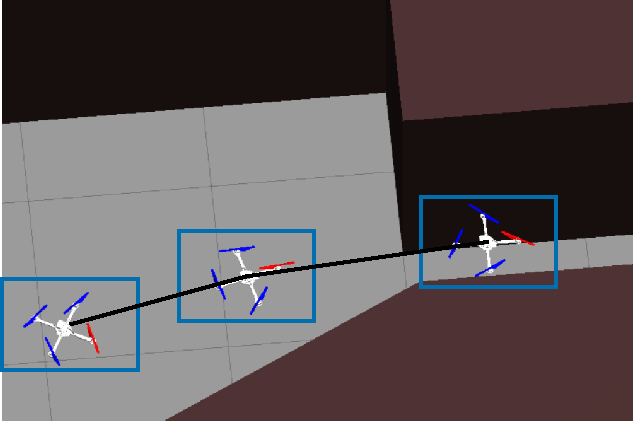
\includegraphics[width=\textwidth]{paper2/images/gazebo_res3.pdf}
    \caption{Transform to line formation}
    \label{fig:1gazebo_3}
    \end{subfigure}
    \begin{subfigure}[b]{0.48\textwidth}
    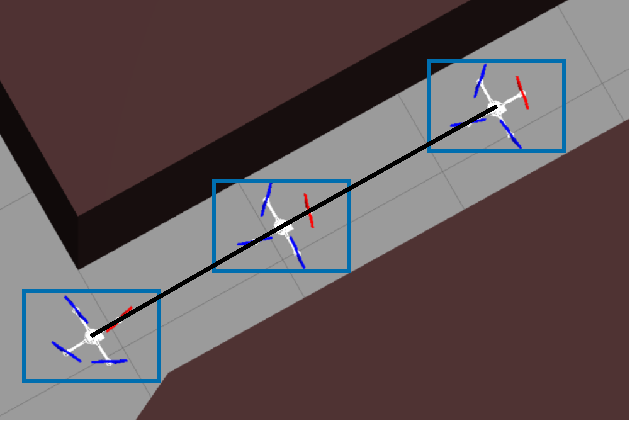
\includegraphics[width=\textwidth]{paper2/images/gazebo_res4.pdf}
    \caption{Line formation}
    \label{fig:1gazebo_4}
    \end{subfigure}
    \begin{subfigure}[b]{0.48\textwidth}
    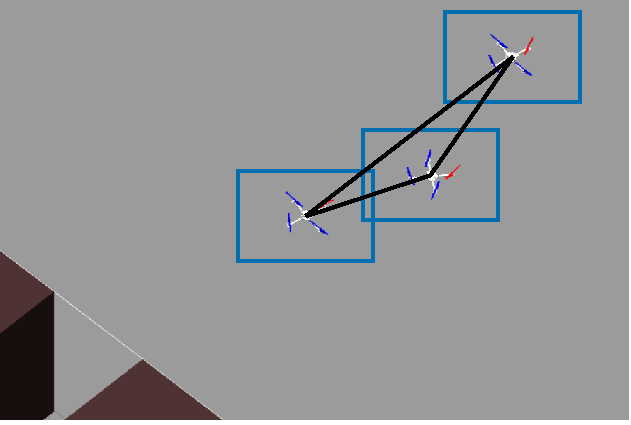
\includegraphics[width=\textwidth]{paper2/images/gazebo_res5.pdf}
    \caption{Transform back to triangle formation}
    \label{fig:1gazebo_5}
    \end{subfigure}
    \begin{subfigure}[b]{0.48\textwidth}
    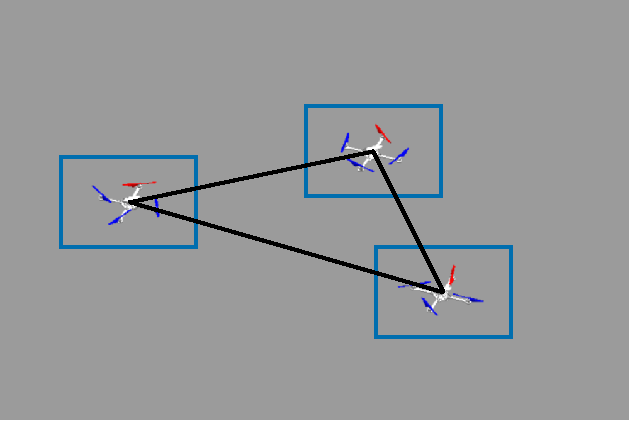
\includegraphics[width=\textwidth]{paper2/images/gazebo_res6.pdf}
    \caption{Original triangle formation}
    \label{fig:1gazebo_6}
    \end{subfigure}
    \caption{Validation results captured in the SIL Gazebo}
    \label{fig:1gazebo_result}
\end{figure*}

\begin{figure*}
    \centering
    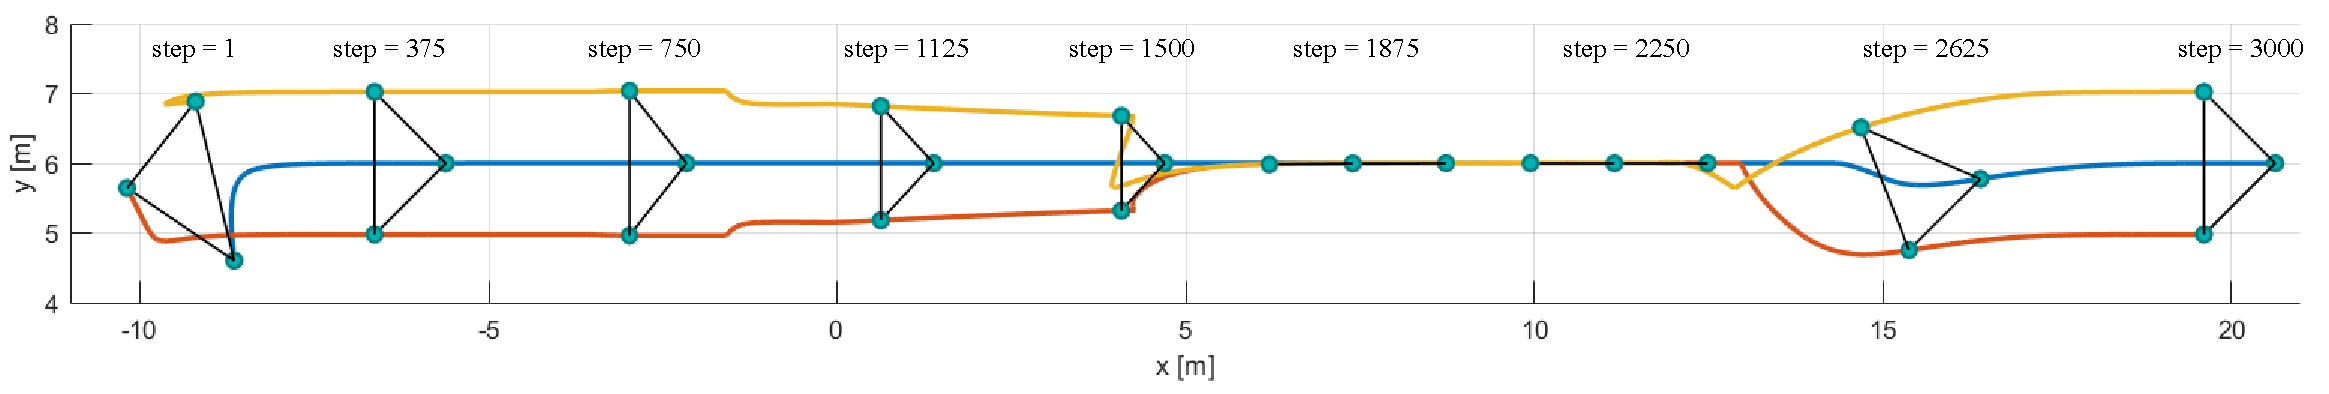
\includegraphics[width=\textwidth]{paper2/images/gazebo_path.pdf}
    \caption{The recorded paths of three UAV in the SIL test (Top view)}
    \label{fig:1gazebo_path}
\end{figure*}

To evaluate the applicability of the proposed system, we have conducted a software-in-the-loop (SIL) validation that involves navigating UAV formation pass through a confined space, which only focuses on a narrow tunnel-like environment in a Gazebo\footnote{Gazebo experiment video: {\fontfamily{qcr}\selectfont
\url{https://youtu.be/AIAAzRiIepg}}}. The used UAV model is a Hummingbird quadrotor developed based on Gazebo-based RotorS simulator~\cite{Furrer2016}, as described in Fig.~\ref{fig:1gazebo_uav}. We set up three UAVs in the experiment with random positions, as shown in Fig.~\ref{fig:1gazebo_init}. The environment in the SIL test includes two large obstacles, forming a width-varying tunnel, as depicted in Figure \ref{fig:1gazebo_env}.

Fig.~\ref{fig:1gazebo_result} presented the formation moving captured in the experiment. Moreover, the paths of three UAVs in the SIL test are recorded and are depicted in Fig.~\ref{fig:1gazebo_path}. At the beginning of the motion (step 1), three UAVs are in the random position. They then move to form the desired triangle formation (steps 375 - 750), as shown in Fig.~\ref{fig:1gazebo_1}. When sensing the narrow passage, the formation shrinks to safely move through the passage (steps 1125 - 1500), as shown in Fig.~\ref{fig:1gazebo_2}. When the narrow space is not suitable for the original formation, the formation transforms to the straight line formation as Fig.~\ref{fig:1gazebo_3} and then passes through the space with the line formation (steps 1875 - 2550), as Fig.~\ref{fig:1gazebo_4}. Once the UAV senses enough space in the environment to maintain its original formation, the formation transforms back to the origin shape in Fig.~\ref{fig:1gazebo_5} and moves to the target in Fig.~\ref{fig:1gazebo_6} (steps 2625 - 3000). The experiment demonstrates that the proposed \textit{EFRC} strategy successfully navigates the UAVs' formation to the target by passing through the narrow passage.

% \subsection{Discussion}
% Through simulation, validation, comparative statistics, and SIL testing, it is clear that our proposed method is capable of navigating the formation ensuring configuration, safety, and optimality for robot operation in narrow space environment.

% The proposed strategy provides flexibility for the robot formation to move safely through narrow space environments with numerous of formation configuration the ability to scale, rotate, and transform into a line configuration based on the perception of the environment depicted in Figure \ref{fig:1path}.

% The proposed algorithm also ensures scalability across various robot quantities within the formation, as presented in Figure \ref{fig:1path}. As long as the robots adhere to the specified configuration, the strategy offers the flexibility to navigate through narrow environments effectively.

% In our design, the formation maintenance and tailgating behaviors are proven to be stable through Lyapunov's theorem (see Appendix \ref{app:uf} and Appendix \ref{app:ut}), which proves that the system errors will converge to zero, as provided in Figure \ref{fig:1error}. Their convergence speed can be controlled through the parameters, $k_f$, $k_t$.

% On another note, our proposed strategy brings forth the capability to swiftly respond to environmental variations and traverse narrow spaces securely. Nonetheless, the transitions between states and abrupt alterations in formation size may result in occasional movement disruptions (see \textit{order} metric in Figure \ref{fig:1metric}). In such instances, employing control techniques like fuzzy logic or neural networks can be employed to improve the overall fluidity of formation movement.
\section{Conclusion}\label{sec5}
In this study, we have presented an event-based reconfiguration control to navigate a time-varying robot formation through narrow spaces across various environmental settings, including forest-like and tunnel-like terrains. The proposed strategy is constructed via several behaviors, which leverage the artificial potential field, which brings t to facilitate implementation. The controller includes two modes, \textit{``formation''} and \textit{``tailgating''}, and a scaling factor that enables the TVF to adapt its shape based on observed environmental conditions. The stability of the proposed approach is also demonstrated via the Lyapunov theorem. Evaluation results show that the proposed controller effectively navigates complex environments, achieving superior control performance in most metrics compared to other established methods. Additionally, software-in-the-loop tests verify the practicality and robustness of the proposed controller in real-world scenarios.


\chapter{Predictive Reconfiguration Control for Multi-Robot Formation in Cluttered Environments}\label{paper3}

\noindent{\normalsize Submitted in:\\
\textit{IEEE Transactions on Control of Network Systems}, 2024\\
Code: {\tt\url{https://github.com/duynamrcv/prc}}\\
Video: {\tt\url{https://youtu.be/oAhgOOhFSCA}}
}
\vspace{1cm}

\noindent\textit{\textbf{Abstract}}

Reconfiguration control is essential for multi-robot systems to adapt their formations in response to environmental conditions when carrying out complex tasks. This paper introduces a novel approach called predictive reconfiguration control (PRC) to navigate a swarm of robots through cluttered environments with narrow passages such as valleys or tunnels. The robot swarm is modeled as a directed sensing graph where each node represents a robot capable of collecting real-time data on the environment and the states of nearby robots within its communication range. The information from each node is used as input to the controller to adjust its parameters in two control modes, \textit{``formation''} and \textit{``tailgating''}, which serve as the basis for formation adaptation. A set of cost functions is then introduced to represent swarm constraints, including formation shape, reference speed, movement direction, and collision avoidance. These cost functions also allow for the prediction of the swarm's states so that model predictive control solvers can be used to minimize the cost for optimal control signals. Results from a number of comparisons and evaluations show that the proposed controller is not only capable of navigating the robot swarm through challenging environments with narrow passages but also outperforms other state-of-the-art formation control techniques in most performance metrics. Software-in-the-loop tests have been conducted to verify the validity of the proposed controller for practical scenarios.
% \end{abstract}

\noindent\textbf{\textit{Keywords:}}
formation control, multi-robot system, distributed control, reconfiguration control, model predictive control
% \end{keywords}

\section{Introduction}
Formation control of multiple robots is becoming increasingly important due to its capability to perform challenging tasks in complex environments such as disaster response, search and rescue, tracking of multiple targets, and swarm-based reconnaissance~\cite{9306908,Oh2015}. This approach also enhances system resilience as any malfunction within the swarm can be mitigated by reconfiguring the formation. The reconfiguration also enables the swarm to navigate through cluttered environments where a fixed topology is insufficient to adapt the formation to varying conditions. Formation reconfiguration control therefore is essential to ensure the effective operation of a robot swarm.

In formation control, a popular approach is based on natural collectives, such as school of fish or flocking of birds~\cite {Nagy2010}, where movement is driven by a set of simple behaviors: \textit{repulsion} that steers an agent away from its neighbors; \textit{cohesion} that attracts the agent to the group; \textit{migration} that orients its motion in a preferred direction; and \textit{obstacle repulsion} to avoid collisions~\cite{Reynolds1987}. Those behaviors are often used with artificial potential fields (APF) to produce control signals for each robot~\cite{736776,Berlinger2021,9565893, 7434587}. In particular, formation and navigational behaviors are combined in~\cite{736776} as concurrent asynchronous processes to guide a group of robots to reach their goals in a desired formation. In~\cite{Berlinger2021}, the AFP is used to coordinate behaviors among fish-inspired miniature underwater robots to obtain  
collective capabilities without having direct communication. However, behavior-based methods are limited in guiding the swarm through complex environments because a set of fixed behaviors lack the flexibility to handle abrupt changes in the environment~\cite{Zhang2023}.

To address this limitation, several studies propose a hybrid approach that combines the AFP with optimization techniques to better integrate behaviors. For example, the APF is used with an artificial neural network in~\cite{Elkilany2020} to optimize potential force parameters so that the swarm can adapt to environmental conditions. Similarly, an evolutionary optimization framework is introduced in \cite{Vsrhelyi2018} to select parameters and fitness functions that enhance the velocity and cohesion of the swarm. Nevertheless, optimizing parameters is insufficient to address the main problem of the behavior-based approach, which depends on a set of fixed behaviors. 

Recently, an approach using optimal control to manage swarm constraints and predict agents' states has been introduced for reliable formation~\cite{Beaver2021,Soria2021,8950150}. In~\cite{7828016,Wu2020}, optimization-based motion planners are used for individual point-to-point transitions to maintain the formation shape while avoiding collisions in multi-robot systems. In~\cite{Soria2021}, model predictive control (MPC) is introduced for swarm navigation in which cost functions and constraints are used to regulate speed, ensure safety, and guide the drones through the environment. The system however is centralized and dependent on a primary agent. A distributed MPC in~\cite{9562281} offers decentralized computation for formation control, but it is only practical in spacious cluttered environments. Maintaining a specific formation shape in tight spaces is challenging due to conflicts between shape preservation and collision avoidance. 

In another direction, several studies propose control techniques that reconfigure the formation in response to sudden changes in the environment structure \cite{AlonsoMora2018,9013071,9981858,10417519}. In~\cite{AlonsoMora2018}, a distributed method capable of reconfiguring the formation is introduced for environments with both static and dynamic obstacles. The method computes a movable convex region from the robots' current positions and then repositions them within this region based on the desired movement direction. However, the transition relies on reassigning robots to predefined virtual points on the reference formation rather than utilizing information obtained from the environment. In~\cite{9981858}, affine transformations are used to modify formation shapes for obstacle avoidance in dense environments, but they require information to be shared among all the robots. Our previous work~\cite{10417519} adapts a V-shape formation to guide a robot swarm through narrow corridors. The two wings of the V-shape can expand or contract to form a suitable shape based on real-time information about the available space. Nonetheless, this approach has not considered the physical limits of the robots, which could lead to infeasible control inputs and unexpected collisions in certain scenarios. Besides, the ability of each robot to make decisions based on local sensor data remains limited.

Building upon recent progress in multi-robot formation, this work introduces a novel technique named predictive reconfiguration control (PRC) for safe and effective navigation of a decentralized multi-robot swarm in cluttered environments. The robots are equipped with local sensors and communication modules to collect information about the environment and the states of their neighboring robots. The PRC is implemented on each robot to enable adaptive formation capabilities. The contributions of this work are threefold:
\begin{enumerate}
    \item Model the formation as a directed sensing graph where each node represents a robot capable of sensing its surroundings and communicating with its neighbors. This representation allows the system to be decentralized and the formation to be formulated as an optimization problem.
    \item Define a set of cost functions that represent the formation constraints and performance. The functions ensure not only the desired formation shape but also the swarm's performance, including the desired velocity, direction, and obstacle avoidance. The cost functions are designed to be compatible with existing solvers for MPC, thereby simplifying the implementation.
    \item Propose a predictive reconfiguration controller with two modes, \textit{``formation''} and \textit{``tailgating''}, capable of adapting the formation shape in response to environmental changes. Extensive simulations and comparisons have been conducted to evaluate the robustness, scalability, and effectiveness of the proposed controller. Software-in-the-loop tests have also been conducted to verify its practical applicability. The source code of the proposed controller is publicly available for further research and practical implementation.
\end{enumerate}

The remaining sections of this chapter are organized as follows. Section~\ref{sec:problem} describes the formation model. Section~\ref{sec:propose} presents the proposed formation reconfiguration control method. Section~\ref{sec:result} shows simulations, comparisons, and software-in-the-loop experimental results. The paper ends with conclusions drawn in Section~\ref{sec:conclusion}.

\section{Formation Background}\label{sec:problem}
Consider a swarm $\mathcal{N}$ of $N$ robots labeled $i\in\left\{1,...,N\right\}$. The swarm is modeled as a directed sensing graph $\mathcal{G}=\left(\mathcal{V},\mathcal{E}\right)$, where vertex set $\mathcal{V} = \left\{1,..., N\right\}$ represents the robots, and edge set $\mathcal{E}\subseteq\mathcal{V}\times \mathcal{V}$ includes robot pairs $\left(i, j\right)\in\mathcal{E}$ for which robot $i$ can sense robot $j$. Denote $\mathcal{N}_i=\left\{j\in\mathcal{V}|\left(i,j\right)\in\mathcal{E}\right\}\subset\mathcal{V}$ as the set of $N_i$ neighbors of a robot $i$ in $\mathcal{G}$.

In this work, the dynamics of the robots are represented in discrete time. Denote $p_i(k),v_i(k),u_i(k)\in\mathbb{R}^3$ respectively be the position, velocity and control input of robot $i$ at time $t(k) = k\tau$, where $\tau$ is the sampling period. The robots in the swarm are homogeneous with a body radius $r$. Each robot is equipped with an inertial measurement unit (IMU) to determine its position and orientation, a range sensor to scan the environment, and a wireless ad-hoc network module to carry out peer-to-peer communication with other robots. In this work, the communication delay between each pair of robots is negligible~\cite{AlonsoMora2018,9527169}. The range sensor provides a $360^\circ$ field of view with the scanning area $S_s$ of radius $r_s$, as shown in Figure~\ref{fig:model}. Its point data obtained at time $t(k)$ is represented by set $\mathcal{M}_i(k)=\left\{m\right\}$.
\begin{figure}
    \centering
    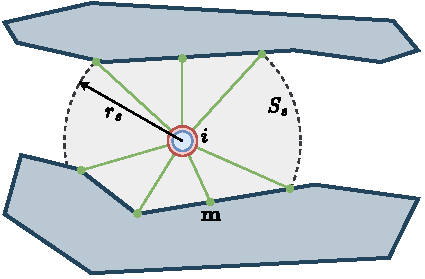
\includegraphics[width=0.48\textwidth]{paper3/images/model.pdf}
    \caption{Illustration of a robot with its range sensor having the scanning area $S_s$ (dashed gray circle) of radius $r_s$ and set $\mathcal{M}_i=\{m\}$ (green) of the acquired point data.}
    \label{fig:model}
\end{figure}

According to~\cite{Soria2021}, the robot in the swarm can be represented as a discrete linear system as follows:
\begin{equation}
    x_i(k+1)=A_ix_i(k) + B_iu_i(k),
\end{equation}
where $A_i$ and $B_i$ are system matrices, $u_i$ is input acceleration, and $x_i=\left[p_i;v_i\right]\in\mathbb{R}^6$ is a state vector including position and velocity. The velocities and accelerations are bounded, i.e., $v_\text{min}\leq v_i(k)\leq v_\text{max}$ and $u_\text{min}\leq u_i(k)\leq u_\text{max}$.
\section{Predictive Reconfiguration Control}\label{sec:propose}

\begin{figure}
    \centering
    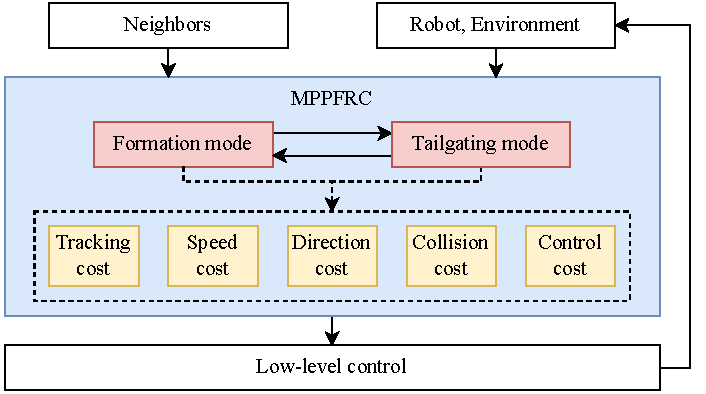
\includegraphics[width=0.7\textwidth]{paper3/images/diagram.pdf}
    \caption{Diagram of the proposed predictive reconfiguration control strategy.}
    \label{fig:diagram}
\end{figure}

The aim of reconfiguration control is to drive the robot swarm through a cluttered environment having narrow passages. The swarm adheres to the following constraints: (\textit{C1}) maintain certain desired shapes; (\textit{C2}) move along a prioritized direction $\mathbf{u}_\text{ref}\in\mathbb{R}^{3}$; (\textit{C3}) obtain the desired speed $\bar{v}_\text{ref}\in\mathbb{R}$; and (\textit{C4}) ensure no collision with other neighbors or obstacles in the environment. To address this problem, we propose a predictive reconfiguration control system as shown in Figure~\ref{fig:diagram}. Inputs to this system include point cloud data from range sensors and the states of neighbor robots. Depending on the environment structure inferred from the point cloud data, the controller operates in either the \textit{``formation''} or \textit{``tailgating''} mode. The \textit{``formation''} mode maintains the desired shape, whereas the \textit{``tailgating''} mode transforms the formation into a line to navigate through narrow spaces like valleys or tunnels. The controller is designed based on a weighted-sum of five cost functions to meet constraints $(C1)-(C4)$. An optimal solver is then used to generate control signals for low-level controllers.

Let $\delta_{ij}\in\mathbb{R}^3,\forall j\in \mathcal{N}_i$ be the vector representing the desired position of robot $i$ with respect to neighbor $j$. The formation is obtained via the following constraint~\cite{Dong2016,6798711}:
\begin{equation}
    \lim_{k\to\infty}{\left(\mathbf{p}_j(k)-\mathbf{p}_i(k)+\kappa\delta_{ij}\right)}=0,\quad\forall i,j\in\{1,...,n\}, i\neq j
\end{equation}
where $\kappa\in[0,1]$ is a scaling factor representing the shrinkage level of the formation. The desired relative position of robot $i$ in the formation is then described as:
\begin{equation}
    \mathbf{p}^*_i(k)=\dfrac{1}{n_i}\sum_{j\in\mathcal{N}_i}{\left(\mathbf{p}_j\left(k\right)+\kappa\delta_{ij}\right)}.
    \label{eqn:formation}
\end{equation}

During the transition between modes, each robot determines a leader as a reference to determine its position. The leader is selected based on the inner product $\tilde{\mathbf{p}}_{ij}$ of the difference between robot $j$ in the neighbor set $\mathcal{N}_i$ and robot $i$, $\mathbf{p}_j-\mathbf{p}_i$, and the desired direction, $\mathbf{u}_\text{ref}$, as follows:
\begin{equation}
    \tilde{\mathbf{p}}_{ij} = \left\langle (\mathbf{p}_j-\mathbf{p}_i),\mathbf{u}_\text{ref}\right\rangle.
    \label{eqn:tildep}
\end{equation}

A positive value of $\tilde{\mathbf{p}}_{ij}$ indicates that robot $j$ is in front of robot $i$ in the $\mathbf{u}_\text{ref}$ direction, and vice versa. Let $\mathcal{P}_i$ be the set of inner products for all robots $j$ in the neighbor set $\mathcal{N}_i$, $\mathcal{P}_i=\left\{\tilde{\mathbf{p}}_{ij}\right\}$. Leader robot ${l_i}$ of robot $i$ is chosen as the closest robot in front of it, i.e.,
\begin{equation}
     l_i=\begin{cases}
    \arg\min_{j}\left\{\tilde{\mathbf{p}}_{ij}\in\mathcal{P}_i\vert\tilde{\mathbf{p}}_{ij}\geq0\right\} & \exists~\tilde{\mathbf{p}}_{ij}\geq0\\ 
    -1 & \text{otherwise}
     \end{cases}
    \label{eqn:li}
\end{equation}

\begin{algorithm}
\caption{Pseudocode of the leader selection}
\label{alg:ls}
\ForEach{$j\in\mathcal{N}_i$}{
    Compute inner product $\tilde{\mathbf{p}}_{ij}$\tcc*[r]{Eq. \ref{eqn:tildep}}
    $\mathcal{P}_i\leftarrow\tilde{p}_{ij}$\;
}
Select leader $l_i$ for robot $i$ to follow\tcc*[r]{Eq. \ref{eqn:li}}
\Return $l_i$\;
\end{algorithm}

Algorithm~\ref{alg:ls} presents the leader selection process. 

In the \textit{``tailgating''} mode, robot~$i$ needs to align and keep a distance~$d_\text{ref}\in\mathbb{R}$ with its leader~$l_i$. This can be formulated as follows:
\begin{equation}
    \lim_{k\to\infty}{\left\Vert \mathbf{p}_{l_i}(k)-\mathbf{p}_i(k)\right\Vert}=d_\text{ref}
    \label{eqn:tailcon}
\end{equation}
The desired relative position of robot~$i$ then can be determined as follows:
\begin{equation}
    \mathbf{p}_i^*(k)= \mathbf{p}_{l_i}(k)-d_\text{ref}\mathbf{u}_\text{ref}.
    \label{eqn:tailgating}
\end{equation}

Using equations \eqref{eqn:tildep} and \eqref{eqn:tailgating}, the formation problem is converted into tracking the desired position $\mathbf{p}_i^*$, which can be handled by predictive controllers. 

\subsection{Predictive control design} 
\begin{figure*}
    \centering
    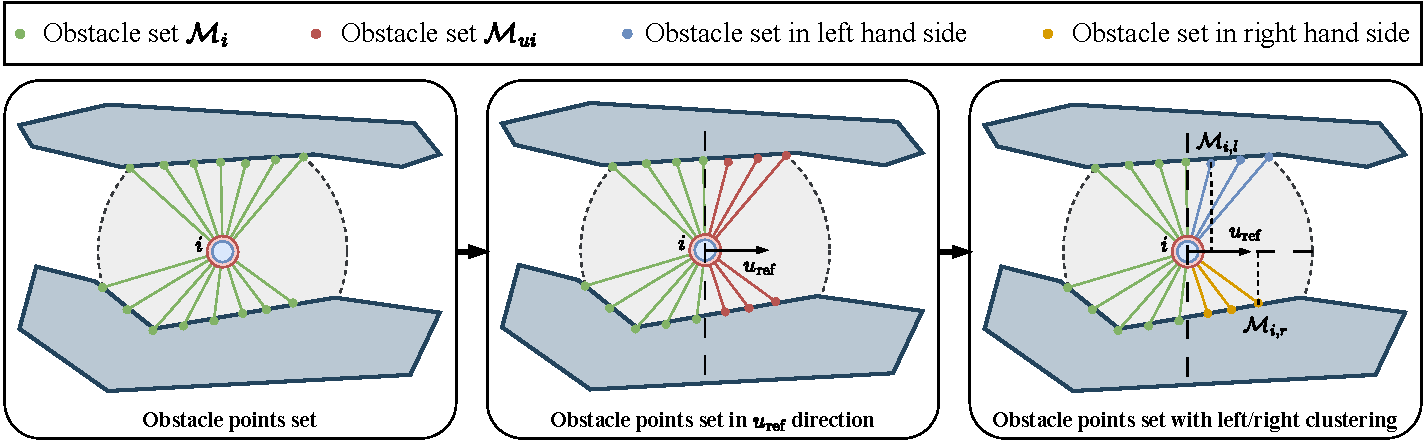
\includegraphics[width=\textwidth]{paper3/images/perception.pdf}
    \caption{The process of estimating the environment's width from the robot's range sensor.}
    \label{fig:perception}
\end{figure*}
The proposed predictive controller uses the desired position $\mathbf{p}_i^*$ as the reference and a set of cost functions to fulfill formation constraints $(C1)-(C4)$. The functions include tracking cost $J_{t,i}$, direction cost $J_{d,i}$, speed cost $J_{s,i}$, obstacle avoidance cost $J_{o,i}$, inter-agent collision cost $J_{i,i}$, and control effort cost $J_{u,i}$. Let $P\in\mathbb{N}^+$ be the prediction horizon, which is finite and shifts forward at each time step; $(\cdot)(k+l|k )$, $l \in\{0,...,P\}$, be the predicted value of $(\cdot)(k+l )$ when the information at time $t(k)$ is available; $\mathbf{X}_i(k)\in\mathbb{R}^{6P}$ be the sequence of the predicted states $\mathbf{x}_i(k+l|k)$ over the horizon $l\in\{1,...,P\}$; and $\mathbf{U}_i(k)\in\mathbb{R}^{3P}$ be the sequence of the predicted control inputs $\mathbf{u}_i(k)$ over the horizon $l\in\{0,...,P-1\}$. The predictive reconfiguration control can be modeled as a non-convex optimization problem as follows:
\begin{equation}
    \min_{\mathbf{U}_i(k)}\left(J_{t,i}(k)+J_{s,i}(k)+J_{d,i}(k)+J_{o,i}(k)+J_{i,i}(k)+J_{u,i}(k)\right)
    \label{eqn:J}
\end{equation}
subject to:
\begin{equation}
    \begin{aligned}
        &\mathbf{x}_i(k+l+1|k)=\mathbf{A}\mathbf{x}_i(k+l|k)+\mathbf{B}\mathbf{u}_i(k+l|k),\\
        &\mathbf{x}_i(k|k)=\mathbf{x}_i(k),\\
        &\mathbf{v}_\text{min}\leq \mathbf{v}_i(k+l|k)\leq \mathbf{v}_\text{max},\\
        &\mathbf{u}_\text{min}\leq \mathbf{u}_i(k+l|k)\leq \mathbf{u}_\text{max},\\
    \end{aligned}
    \label{eqn:constraints}
\end{equation}
with $l\in\{1,...,P\}$, and $i\in\mathcal{N}$. The cost functions are defined as follows.

\subsubsection{Tracking cost}\label{sec:tracking_term}
The tracking term aims to drive the robots toward their reference positions to achieve the desired formation shape. It is defined as the square error between the desired position~$\mathbf{p}_i^*$ and the predicted position~$\mathbf{p}_i$ of robot $i$ as follows:
\begin{equation}
    J_{t,i}(k)=w_t\sum_{l=1}^P{\left\Vert \mathbf{p}^*_i(k+l|k)-\mathbf{p}_i(k+l|k)\right\Vert^2},
\end{equation}
where $w_t$ is a positive tracking weight.

\subsubsection{Speed cost}
The speed cost is used to maintain the desired speed $v_\text{ref}$ of the swarm. It is defined as the squared difference between the actual and the desired speed of the robots as follows:
\begin{equation}
    J_{s,i}(k)=w_s\sum_{l=1}^P\left(\left\Vert \mathbf{v}_i(k+l|k)\right\Vert^2-v_\text{ref}^2\right)^2,
\end{equation}
where $w_s$ is a positive weight.

\subsubsection{Direction cost}
This cost directs the robots to move in the desired direction $\mathbf{u}_\text{ref}$. It is computed based on the normalized dot product between velocity $\mathbf{v}_i$ and the desired direction $\mathbf{u}_\text{ref}$ of robot~$i$. It is equal to zero when the velocity perfectly aligns with the reference direction and otherwise increases proportionally with the degree of misalignment. It is given as follows:
\begin{equation}
    J_{d,i}(k)=w_d\sum_{l=1}^P{\left(1-\dfrac{\left\langle \mathbf{v}_i\left(k+l|k\right),\mathbf{u}_\text{ref}\right\rangle^2}{\left\Vert \mathbf{v}_i(k+l|k)\right\Vert^2}\right)^2},
\end{equation}
where $w_d$ is a positive direction weight.

\subsubsection{Collision avoidance cost}
To avoid collisions, the distance from a robot to any obstacle must be greater than the robot's radius $r$ and the distance between any two robots must be greater than $2r$. Let $d_{ij}=\left\Vert \mathbf{p}_j-\mathbf{p}_i\right\Vert$ be the distance between robots $i$ and $j$, and $d_{im}$ be the distance between robot $i$ and obstacle $\mathbf{m}$. The constraints for collision avoidance  are given as follows:
\begin{equation}
\begin{aligned}
    d_{im}(k+l|k)&\geq r \quad i\in\mathcal{N}, \mathbf{m}\in\mathcal{M}_i(k)
    \label{eq:obsContraint}
\end{aligned}
\end{equation}
\begin{equation}
\begin{aligned}
    d_{ij}(k+l|k)&\geq 2r \quad i\in\mathcal{N},j\in\mathcal{N}_i
    \label{eq:robotContraint}
\end{aligned}
\end{equation}

In this work, constraint (\ref{eq:obsContraint}) is represented via obstacle avoidance cost $J_{o,i}$ defined as a logistic function as follows~\cite{8202163}:   

\begin{equation}
    J_{o,i}(k) = w_o\sum_{l=1}^P \dfrac{1}{1 + \exp{\left(\alpha\left(d_{im}^\text{min}(k+l|k) - r\right)\right)}},
\end{equation}
where $w_o > 0$ is a constant weight, $\alpha > 0$ is a smoothness parameter, and
\begin{equation}
    d_{im}^\text{min}(k+l|k)=\min\left\{d_{im}(k+l|k)|\mathbf{m}\in\mathcal{M}_i\right\}.
\end{equation}

Similarly, constraint (\ref{eq:robotContraint}) is represented via an inter-agent collision cost $J_{i,i}$ defined as follows~\cite{736776}:
\begin{equation}
    J_{i,i}(k)=\dfrac{w_i}{n_i}\sum_{l=1}^P{\sum_{j\in\mathcal{N}_i}}F_{ij}(k+l|k),
\end{equation}
where $w_i>0$ is a constant weight and  
\begin{equation}
    F_{ij}(k+l|k)=\begin{cases}
        0   & \text{if } d_{ij}(k+l|k) \geq \beta r\\
        \dfrac{\beta r-d_{ij}(k+l|k)}{(\beta-2)r}    & \text{if } 2r < d_{ij}(k+l|k) < \beta r\\
        \infty  & \text{if } d_{ij}(k+l|k) \leq 2r
    \end{cases}
\end{equation} 
with $\beta>2$ being the influence ratio of the neighbors.

\subsubsection{Control effort cost}
The control effort cost is used as a penalty term to minimize the control signal. It is defined as:
\begin{equation}
    J_{u,i}(k)=w_u\sum_{l=0}^{P-1}\left\Vert \mathbf{u}_i(k+l|k)\right\Vert^2,
\end{equation}
where $w_u>0$ is a constant control weight.

\subsection{Formation reconfiguration}\label{sec:obs_aware}

Depending on the environment's width, the control system can determine the formation shape and scaling factor $\kappa$. The process of estimating the environment's width is illustrated in Figure~\ref{fig:perception}. Robot $i$ first obtains point cloud data $\mathcal{M}_i$ (green) from its local sensor and then selects a point set $\mathcal{M}_{ui}$ (red) in front of the robot along the moving direction $u_\text{ref}$ as follows:
\begin{equation}
    \mathcal{M}_{ui} = \left\{\mathcal{M}_{i}\vert\left\langle\left(\mathbf{p}_i-\mathcal{M}_{i}\right),u_\text{ref}\right\rangle<0\right\}.
    \label{eqn:mui}
\end{equation}
The DBSCAN algorithm~\cite{10.5555/3001460.3001507} is then used to divide $\mathcal{M}_{ui}$ into two clusters corresponding to the left (blue) and right (yellow) sides of the robot. Data points $\mathcal{M}_{i,l}$ and $\mathcal{M}_{i,r}$ from those clusters with the shortest distance to $u_\text{ref}$ are then selected. Using these points, the environment's width is computed as:
\begin{equation}
    w_e= \left\Vert\left(\mathcal{M}_{i,r}-\mathcal{M}_{i,l}\right)\times \mathbf{u}_\text{ref}\right\Vert
    \label{eqn:we}
\end{equation}
The pseudocode to estimate the environment's width is presented in Algorithm~\ref{alg:we}. 

On the other hand, the formation's width $w_f$ is predefined for each specific formation shape. The scaling factor $\kappa$ then can be computed based on the environment's and formation's width as follows:
\begin{equation}
    \kappa = 
    \begin{cases} 
        \dfrac{w_e - 2r}{w_f} & \text{if } w_e \geq \lambda r \\
        0 & \text{otherwise}
    \end{cases}
    \label{eqn:kappa}
\end{equation}
where $\lambda > 2$ is a scaling coefficient determining the environment's width at which the PRC switches its mode. 

\begin{algorithm}[h!]
\caption{Pseudocode to estimate the environment's width}
\label{alg:we}
Get point set $\mathcal{M}_{ui}$ in front of robot $i$ in moving direction $\mathbf{u}_\text{ref}$\tcc*[r]{Eq. \ref{eqn:mui}}
Cluster $\mathcal{M}_{ui}$ for the left and right sides of the robot using DBSCAN\;
Find point pair $\left(\mathcal{M}_{i,l},\mathcal{M}_{i,r}\right)$, whose distance to $\mathbf{u}_\text{ref}$ is minimum\;
Compute the environment's width $w_e$\tcc*[r]{Eq. \ref{eqn:we}}
\Return $w_e$\;
\end{algorithm}

\begin{algorithm}[h!]
\caption{Pseudocode of the PRC}
\label{alg:our}
Get data point set $\mathcal{M}_i$\;
\If{$\mathcal{M}_i$ is empty}{
    mode $\leftarrow$ \textit{``formation''}\;
    $\kappa \leftarrow 1.0$\;
}
\Else{
    Get the environment's width $w_e$\tcc*[r]{Alg. \ref{alg:we}}
    \If{$w_e$ is None}{
        mode $\leftarrow$ \textit{``formation''}\;
        $\kappa \leftarrow 1.0$\;
    }
    \Else{
        \If{$w_e\leq\lambda r$}{
            mode $\leftarrow$ \textit{``tailgating''}\;
        }
        \Else{
            mode $\leftarrow$ \textit{``formation''}\;
            Estimate the desired formation width $w_f$\;
            \If{$w_e-2r\leq w_f$}{
                Compute the scaling factor $\kappa$\tcc*[r]{Eq. \ref{eqn:kappa}}
            }
            \Else{
                $\kappa\leftarrow1.0$\;
            }
        }
    }
}
\Switch{mode}{
\Case{``formation''}
{
    Get the desired position $\mathbf{p}_i^*$\tcc*[r]{Eq. \ref{eqn:formation}}
}
\Case{``tailgating''}
{
    Select a leader to follow\tcc*[r]{Alg. \ref{alg:ls}}
    Get the desired position $\mathbf{p}_i^*$\tcc*[r]{Eq. \ref{eqn:tailgating}}
}
}
Establish the formation cost function\tcc*[r]{Eqs. \ref{eqn:J}-\ref{eqn:constraints}}

Minimize the cost function to obtain the optimal control signal $\mathbf{u}_i^*$\tcc*[r]{MPC solver~\cite{2020SciPy-NMeth}}

\Return $\mathbf{u}_i^*$\;
\end{algorithm}

Algorithm~\ref{alg:our} presents the pseudocode of the PRC. At each time step, the system estimates the width of the environment to determine the formation mode and the scaling factor $\kappa$. It then computes the desired position $\mathbf{p}_i^*$ for each robot and establishes the formation cost function using equations \eqref{eqn:J} - \eqref{eqn:constraints}. This problem is then solved to find the optimal control signal $\mathbf{u}_i^*$ using common nonlinear programming (NLP)
solvers, such as the Sequential Least Squares Programming (SLSQP)~\cite{kraft1988software}. In this work, we implemented the solver in Python using the optimization software library SciPy~\cite{2020SciPy-NMeth}.
\section{Results and Discussion}\label{sec:result}

\begin{figure*}
    \centering
    \begin{subfigure}[b]{0.495\textwidth}
    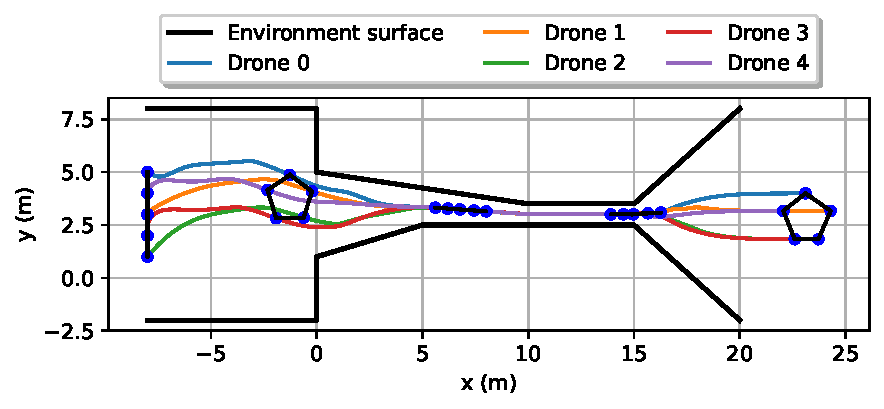
\includegraphics[width=\textwidth]{paper3/images/path_scen1.pdf}
    \caption{Scenario 1 - Motion paths}
    \end{subfigure}
    \begin{subfigure}[b]{0.495\textwidth}
    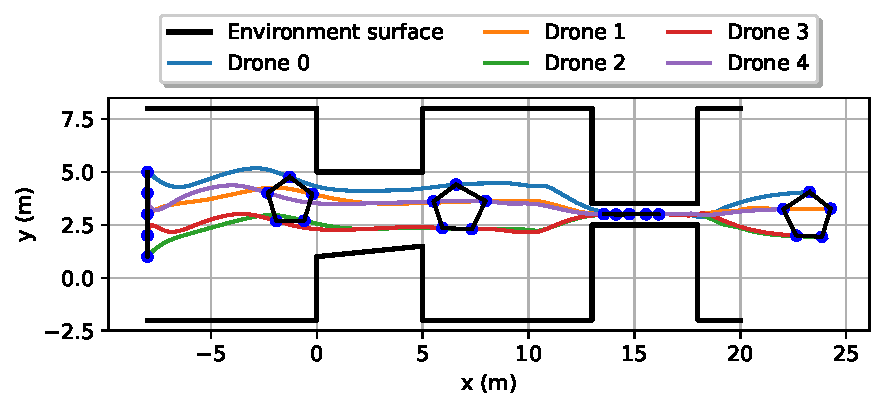
\includegraphics[width=\textwidth]{paper3/images/path_scen2.pdf}
    \caption{Scenario 2 - Motion paths}
    \end{subfigure}
    \begin{subfigure}[b]{0.495\textwidth}
    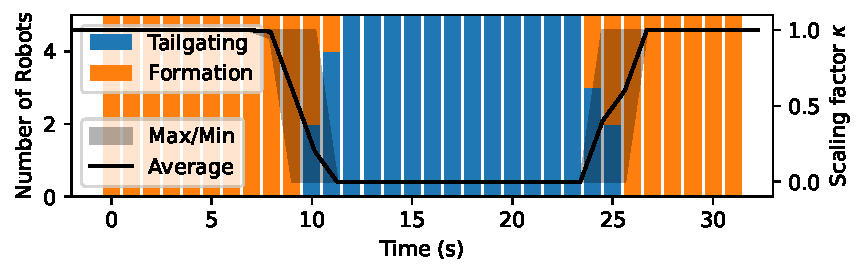
\includegraphics[width=\textwidth]{paper3/images/correlation_scen1.pdf}
    \caption{Scenario 1 - Correlation between the number of  robots (bar chart) in each mode and the scale factor (black line) over time}
    \label{fig:cor1}
    \end{subfigure}
    \begin{subfigure}[b]{0.495\textwidth}
    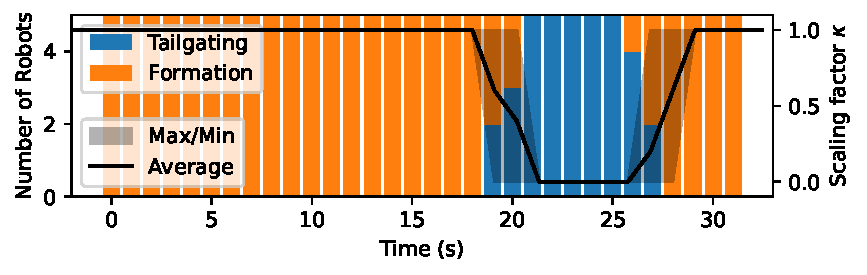
\includegraphics[width=\textwidth]{paper3/images/correlation_scen2.pdf}
    \caption{Scenario 2 - Correlation between the number of  robots (bar chart) in each mode and the scale factor (black line) over time}
    \label{fig:cor2}
    \end{subfigure}
    \caption{Trajectories and formation shapes of the robots controlled by the PRC in two evaluating scenarios.}
    \label{fig:path}
\end{figure*}

A number of simulations, comparisons, and software-in-the-loop tests have been conducted to evaluate the performance of the PRC with details as follows.

\subsection{Evaluation Setup}
The swarm includes five identical robots, each with a radius of $r=0.2$~m, a maximum speed of $\left\Vert v_\text{max}\right\Vert=1.5$~m/s, and a maximum control input $\left\Vert u_\text{max}\right\Vert=2.0$~m/s$^2$. The robot is equipped with a range sensor having the sensing range of $r_s=3$~m. The desired formation shape is set to a pentagon, the reference velocity is $\bar{v}_\text{ref}=1$~m/s, and the desired direction is $u_\text{ref}=[1,0,0]^T$. The environments include two structures, both having narrow passages, as depicted in Figure~\ref{fig:path}.

The metrics used for evaluation include the success rate, mean \textit{order} $\Phi$, mean speed (m/s), mean formation error $\varepsilon$ (m), and acceleration cost $\Gamma$ (m$^2$/s$^4$) \cite{Zhang2021}. The \textit{order} metric~\cite{Vicsek1995} measures the heading consensus of the robots and is computed as:
\begin{equation}
    \Phi=\dfrac{1}{N}\left\Vert\sum_{i=1}^N{\dfrac{v_i}{\left\Vert v_i\right\Vert}}\right\Vert
\end{equation}
Its value ranges from 0 to 1, with 1 indicating the robots have the same direction. The \textit{formation error} measures the deviation between the desired and actual positions of the robots and is calculated as~\cite{6798711}:
\begin{equation}
    \varepsilon_i = \left\Vert p_i-p^*_i\right\Vert
\end{equation} 
The acceleration cost indicates the control effort and is given by:
\begin{equation}
    \Gamma = \dfrac{1}{N}\sum_{i=1}^N{\left\Vert u_i(k)\right\Vert^2}
\end{equation} 

The comparing methods include the behavior-based reconfiguration control (BRC) \cite{Vsrhelyi2018} and the predictive formation control (PFC)~\cite{9562281}. In evaluation, each method is run 10 times for each scenario.   

\subsection{Results}
\label{subsec:results}

\begin{figure*}
    \centering
    \begin{subfigure}[b]{0.495\textwidth}
    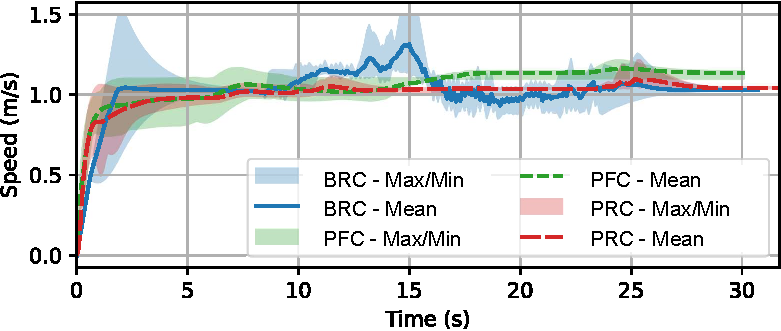
\includegraphics[width=\textwidth]{paper3/images/velocity_scen1.pdf}
    \caption{Scenario 1 - Speed}
    \label{fig:speed1}
    \end{subfigure}
    \begin{subfigure}[b]{0.495\textwidth}
    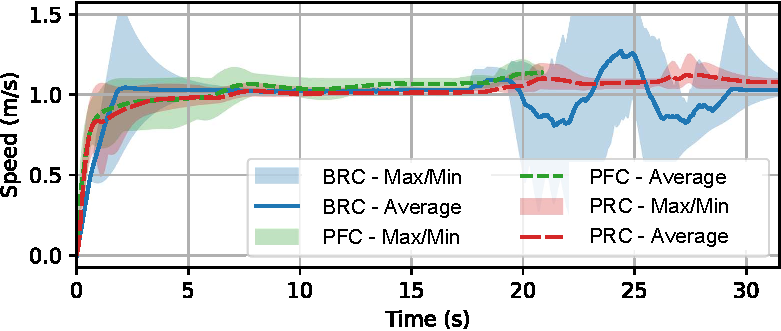
\includegraphics[width=\textwidth]{paper3/images/velocity_scen2.pdf}
    \caption{Scenario 2 - Speed}
    \label{fig:speed2}
    \end{subfigure}
    \begin{subfigure}[b]{0.495\textwidth}
    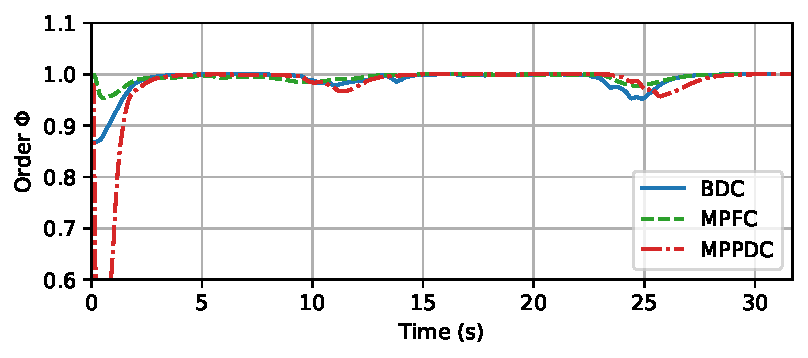
\includegraphics[width=\textwidth]{paper3/images/order_scen1.pdf}
    \caption{Scenario 1 - \textit{Order} $\Phi$}
    \label{fig:order1}
    \end{subfigure}
    \begin{subfigure}[b]{0.495\textwidth}
    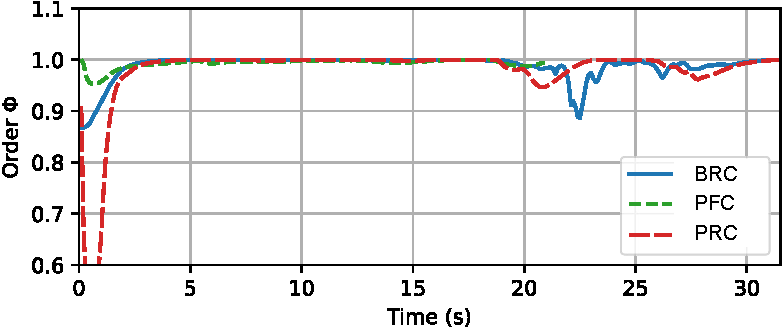
\includegraphics[width=\textwidth]{paper3/images/order_scen2.pdf}
    \caption{Scenario 2 - \textit{Order} $\Phi$}
    \label{fig:order2}
    \end{subfigure}
    \begin{subfigure}[b]{0.495\textwidth}
    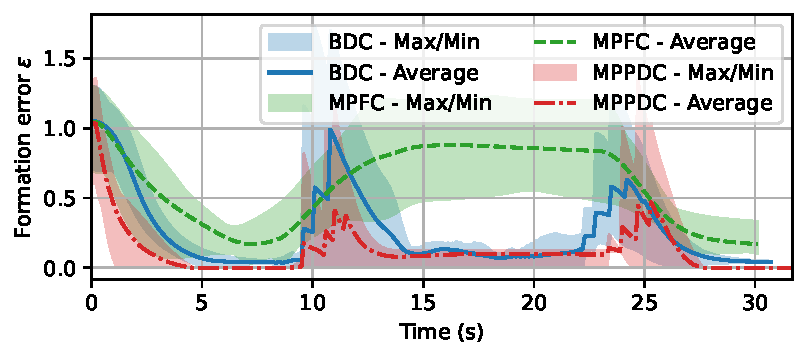
\includegraphics[width=\textwidth]{paper3/images/error_scen1.pdf}
    \caption{Scenario 1 - \textit{Formation error} $\varepsilon$}
    \label{fig:error1}
    \end{subfigure}
    \begin{subfigure}[b]{0.495\textwidth}
    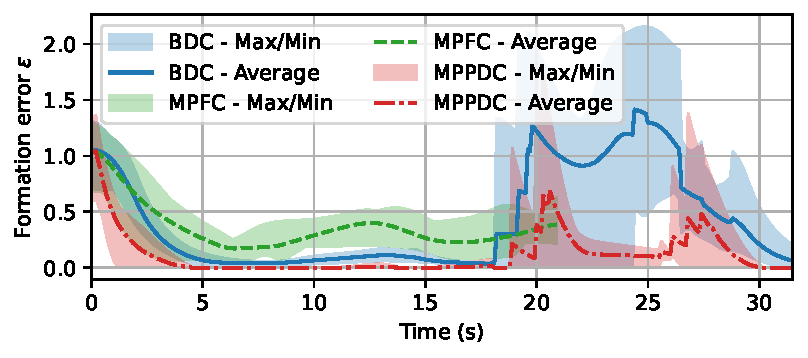
\includegraphics[width=\textwidth]{paper3/images/error_scen2.pdf}
    \caption{Scenario 2 - \textit{Formation error} $\varepsilon$}
    \label{fig:errorr2}
    \end{subfigure}
    \caption{Comparison results of three control methods in two scenarios.}
    \label{fig:comparison}
\end{figure*}

\begin{figure}
    \centering
    \includegraphics[width=0.8\textwidth]{paper3/images/scalability.pdf}
    \caption{Effect of the swarm size on system performance, including the mean \textit{order} $\Phi$ and formation error $\varepsilon$.}
    \label{fig:scalability}
\end{figure}

Figure \ref{fig:path} shows the formation results for both scenarios. After takeoff, the robots rapidly form the desired pentagon shape, then change their formation to pass through tight passages and finally transform back to the original desired shape. Figures~\ref{fig:cor1}-\ref{fig:cor2} depict the scaling factor $\kappa$ and the number of robots within each control mode during operation. When the environment's width is large, the scaling factor $\kappa$ stays at 1 to maintain the desired shape. As the environment narrows, $\kappa$ gradually decreases leading to more robots switching to \textit{``tailgating''} mode. The formation thus shrinks until $\kappa$ reaches 0, the point at which all robots are in \textit{``tailgating''} mode. Upon exiting the narrow corridor, $\kappa$ increases, allowing the formation to expand back to its original shape. The PRC hence provides reconfiguration capabilities for the robot swarm to adapt to complex environmental conditions.

\begin{table*}
\centering
\caption{Comparison between BRC, PFC, and the proposed PRC}
\label{tbl:analys}
\begin{tabular}{C{0.8cm}C{1.2cm}C{1.8cm}C{1.8cm}C{2.8cm}C{2.2cm}C{2.5cm}}
\hline \hline
Scen.             & Method & Success rate  & Mean \textit{order} $\Phi$ & Mean speed (m/s) ($v_\text{ref}=1$~m/s) & Mean formation error $\varepsilon$ (m) & Acceleration cost $\Gamma$ (m$^2$/s$^4$) \\ \hline
\multirow{3}{*}{1  } & BRC      & \textbf{10/10} & 0.9890     & 1.0249     & 0.3048               & 69.6589    \\
                     & PFC     & 8/10  & \textbf{0.9934}     & 1.0639     & 0.6376               & \textbf{23.7442}    \\
                     & PRC    & \textbf{10/10} & 0.9824     & \textbf{0.9863}     & \textbf{0.2423}               & 25.0894    \\ \hline
\multirow{3}{*}{2}   & BRC      & 6/10  & 0.9883     & \textbf{0.9887}     & 0.6872               & 53.8718    \\
                     & PFC     & 0/10  & \textbf{0.9953}     & 1.0470      & 0.4593               & \textbf{19.0365}    \\
                     & PRC    & \textbf{9/10}  & 0.9830     & 0.9800       & \textbf{0.3217}               & 21.8559   \\ \hline \hline
\end{tabular}
\end{table*}
 
Figure~\ref{fig:comparison} presents comparison results between the PRC and other control methods. In terms of speed, the proposed controller achieves more stable velocities with values closer to the reference $v_\text{ref}$ in both scenarios, as indicated via the average and maximum/minimum values shown in Figures~\ref{fig:speed1}-\ref{fig:speed2}. 
For the \textit{order} metric, the PRC exhibits large fluctuation at start but quickly converges to a high consensus among the robots with the \textit{order} value reaching 1, as shown in Figures~\ref{fig:order1}-\ref{fig:order2}. Both the BRC and PFC also perform well, although the BRC shows more variation than the PRC during the transition phase. In terms of formation maintenance, the PRC outperforms other methods with the smallest average error, as shown in Figures~\ref{fig:error1}-\ref{fig:errorr2}. These results are further confirmed in Table~\ref{tbl:analys}, which presents comparison data. The proposed PRC shows high performance in all metrics, with the highest success rate and the smallest formation error in both scenarios. The PFC fails in scenario 2 due to its limitation in reconfiguring the formation. The BRC has good performance in speed and mean order. It however introduces high acceleration costs, indicating that the method is not energy efficient.       

In another experiment, we vary the swarm size between 4, 5, 7, 10, 15, and 20 robots and measure the mean \textit{order} $\Phi$ and formation error $\varepsilon$ to evaluate the scalability of the proposed method. The result in Figure \ref{fig:scalability} shows that as the number of robots increases, the PRC maintains strong consensus among robots with a mean \textit{order} close to~1. The formation error, excluding the formation generation and the transition stage, remains low with variations around 0.05~m. The PRC is therefore scalable with stable performance across different swarm sizes.

\subsection{Software-in-the-loop verification}
\begin{figure*}
    \centering
    \begin{subfigure}[b]{0.56\textwidth}
    \includegraphics[width=\textwidth]{paper3/images/tunnel.pdf}
    \caption{The cave-like environment}
    \label{fig:gazebo_tunnel}
    \end{subfigure}
    \begin{subfigure}[b]{0.42\textwidth}
    \includegraphics[width=\textwidth]{paper3/images/hummingbird.pdf}
    \caption{The drone model~\cite{Bui2022,Furrer2016}}
    \label{fig:gazebo_hummingbird}
    \end{subfigure}
    \caption{The robot and environment structure used for software-in-the-loop tests.}
    \label{fig:sil}
\end{figure*}
\begin{figure*}
    \centering
    \begin{subfigure}[b]{0.325\textwidth}
    \includegraphics[width=\textwidth]{paper3/images/gazebo_01.png}
    \caption{}
    \end{subfigure}
    \begin{subfigure}[b]{0.325\textwidth}
    \includegraphics[width=\textwidth]{paper3/images/gazebo_02.png}
    \caption{}
    \end{subfigure}
    \begin{subfigure}[b]{0.325\textwidth}
    \includegraphics[width=\textwidth]{paper3/images/gazebo_03.png}
    \caption{}
    \end{subfigure}
    \begin{subfigure}[b]{0.325\textwidth}
    \includegraphics[width=\textwidth]{paper3/images/gazebo_04.png}
    \caption{}
    \end{subfigure}
    \begin{subfigure}[b]{0.325\textwidth}
    \includegraphics[width=\textwidth]{paper3/images/gazebo_05.png}
    \caption{}
    \end{subfigure}
    \begin{subfigure}[b]{0.325\textwidth}
    \includegraphics[width=\textwidth]{paper3/images/gazebo_06.png}
    \caption{}
    \end{subfigure}
    \caption{Reconfiguration process of the robot swarm in a SIL test: (a) initial positions of the robots; (b) form the desired pentagon shape; (c) shrink the formation in adaption to the environment; (d)-(e) switch to \textit{``tailgating''} mode to travel through the narrow passage; (f) transform back to the desired shape.}
    \label{fig:snap}
\end{figure*}

\begin{figure*}
    \centering
    \begin{subfigure}[b]{0.48\textwidth}
    \includegraphics[width=\textwidth]{paper3/images/gazebo_path.pdf}
    \caption{The formation and motion paths}
    \label{fig:gazebo_path}
    \end{subfigure}
    \begin{subfigure}[b]{0.48\textwidth}
    \includegraphics[width=\textwidth]{paper3/images/gazebo_correlation.pdf}
    \caption{Number of robots and scaling factor $\kappa$}
    \label{fig:gazebo_mode}
    \end{subfigure}
    \begin{subfigure}[b]{0.48\textwidth}
    \includegraphics[width=\textwidth]{paper3/images/gazebo_speed.pdf}
    \caption{The speed profile}
    \label{fig:gazebo_speed}
    \end{subfigure}
    \begin{subfigure}[b]{0.48\textwidth}
    \includegraphics[width=\textwidth]{paper3/images/gazebo_order.pdf}
    \caption{The \textit{order} metric $\Phi$}
    \label{fig:gazebo_order}
    \end{subfigure}
    \begin{subfigure}[b]{0.48\textwidth}
    \includegraphics[width=\textwidth]{paper3/images/gazebo_error.pdf}
    \caption{The \textit{formation error} $\varepsilon_i$}
    \label{fig:gazebo_error}
    \end{subfigure}
    \begin{subfigure}[b]{0.48\textwidth}
    \includegraphics[width=\textwidth]{paper3/images/gazebo_computation.pdf}
    \caption{The computational time}
    \label{fig:gazebo_time}
    \end{subfigure}
    \caption{Results of the SIL tests}
    \label{fig:gazebo}
\end{figure*}

We have carried out software-in-the-loop (SIL) tests to evaluate the performance of the proposed controller in practical conditions. The environment is a narrow space that consists of two large obstacles forming a cave-like structure as shown in Figure~\ref{fig:gazebo_tunnel}. The robots include five homogeneous Hummingbird quadrotors\footnote{Source code used to setup SIL tests in Gazebo - {\tt\url{https://github.com/duynamrcv/hummingbird_simulator}}} obtained from the RotorS simulator~\cite{Furrer2016} with an arm length of 0.17~m, a mass of 0.716~kg, the rotor thrust constant of $1.6\time10^{-2}$~N/A, and the rotor drag constant of $8.54858\times10^{-6}$~Nm/A, as depicted in Figure~\ref{fig:gazebo_hummingbird}. Each robot is equipped with a range sensor to collect point cloud data of the environment, a positioning module for localization, and a communication module to interact with other robots.

Figure~\ref{fig:snap} presents the formation reconfiguration process as the swarm navigates through the environment. The robots continuously collect data about the environment and based on it adjust their formation to ensure safe operation. Figure~\ref{fig:gazebo} provides a detailed view of the result. Each UAV determines its mode and desired position based on the perception of the surrounding environment and information about its neighbors. The robots together form the relevant shape in a decentralized manner, as shown in Figures~\ref{fig:gazebo_path} - \ref{fig:gazebo_mode}. Requirements for speed, order, and formation accuracy are also met, as depicted in Figures~\ref{fig:gazebo_speed} - \ref{fig:gazebo_error}. Moreover, the computational time per controller iteration, shown in Figure~\ref{fig:gazebo_time}, indicates that the system can operate at a sampling rate of 10 Hz in the worst-case scenario, which is sufficient for real-time robot operation.

\subsection{Discussion}
Evaluation and comparison results show the key properties of the proposed control method as follows:

\subsubsection{Decentralization} The PRC is fully decentralized as each robot makes decisions based solely on its own sensor data and information from its neighbors. Unlike the approach in~\cite{AlonsoMora2018}, which requires system-wide communication to obtain information on all robots, the PRC utilizes only one-hop communication between the robot and its neighbors to update predictive states.

\subsubsection{Reliability}

The PRC can navigate the robots through complex environments with desirable performance metrics such as low formation error, stable formation direction, and high speed. Unlike previous studies ~\cite{Elkilany2020,Vsrhelyi2018,Soria2021,AlonsoMora2018} which only shrink or expand the formation to adapt to environment variations, the PRC enables the robots to completely transform to a new formation to safely maneuver through tight spaces.

\subsubsection{Scalability}
The PRC can operate with different swarm sizes, for example from 4 to 20 robots, without requiring any modifications to the algorithm. It maintains reliable performance and consistent metric values across various swarm sizes. 

\subsubsection{Robustness}
The PRC provides robustness to operate in different environmental structures. Through real-time data obtained from local sensors and communication networks, the swarm can dynamically expand, shrink, or transform into a line shape to optimize its ability to navigate through narrow spaces.
\section{Conclusion}\label{sec:conclusion}
In this work, we have presented an optimal predictive reconfiguration control method to guide a swarm of robots through cluttered environments with varying path widths. The controller features two modes, \textit{``formation''} and \textit{``tailgating''}, and a scaling factor that enable the swarm to adapt its shape to environmental conditions. A set of cost functions is introduced to enforce formation constraints and safety requirements while enabling state prediction for enhanced control performance. Evaluation results show that the proposed controller effectively navigates the robot swarm through complex environments with narrow passages. The control performance is superior in most evaluation metrics compared to two other state-of-the-art methods. Software-in-the-loop tests further confirm the validity and practicability of the proposed controller.



\chapter{Conclusion and Future Works}\label{conclusion}

Driven by the potential impact of multiple UAV systems on numerous missions, such as search and rescue (SAR), this master thesis has presented a set of contributions addressing the autonomous navigation of UAV formations through a confined environment, especially in narrow spaces. A brief summary of the conducted research, the key insights, and contributions are given as follows.

Aiming at the safe navigation of a V-shape formation, \textit{Method 1} addresses formation control by designing a distributed architecture for self-reconfiguration. The proposed method is constructed by several behaviors, that allow a V-shape formation to shrink/expand, which depends on the width of the environment. In a collision-free environment, the method ensures that the shape maintenance and inter-collision-freeness between each pair of UAVs are complete. 

Similarly to our previous work in \textit{Method 1}, \textit{Method 2} also address multi-robot navigation. However, instead of focusing on V-shape formation, the study expands the ability to use various types of configuration. This work presents a reconfiguration control method, named event-based reconfiguration control, which is constructed by several behaviors based on artificial potential fields. The stability of the method is also proven via Lyapunov theory. Thanks to the proposed method, robot formation can navigate safely through a narrow space by changing the scale, or transform to a straight line configuration.

Nevertheless, constraints and limitations of robot systems are not considered in the previous works. As a result, \textit{Method 3} model the reconfiguration control as an optimal problem which considers the limitation of robot systems. The behaviors presented in \textit{Method 2} are converted to objective functions, and the control signal is obtained by minimizing the weighted-sum cost function, subject to constraints. By collecting the data from the environment, the surrounding space is considered to estimate the width of the space. The optimal solution not only ensures the effectiveness of the reconfiguration control but also enhances the safety and collision-free.

In future works, we aim to develop safety-critical reconfiguration control strategies that enhance safe movement and minimize the potential of collision with other robots and environments. Due to narrow spaces, the potential of collision between robots with neighbors or environments becomes considerable. As a result, an improvement related to safety-critical is essential to ensure collision-free. Following this, the non-communication formation reconfiguration control methods can be considered to enhance the autonomy and robustness of the systems. A vision-based perception becomes an effective alternative approach to deal with the mentioned problem.
\chapter*{List of related publications}
\addcontentsline{toc}{chapter}{List of related publications}

\subsection*{Articles}
\textbf{Duy-Nam Bui} and Manh Duong Phung, ``Radial Basis Function Neural Networks for Formation Control of Unmanned Aerial Vehicles,'' in \textit{Robotica}, vol. 42, pp. {1842--1860}, 2024.

Thi Thuy Ngan Duong, \textbf{Duy-Nam Bui}, and Manh Duong Phung, ``Navigation Variable-based Multi-objective Particle Swarm Optimization for UAV Path Planning with Kinematic Constraints,'' in \textit{Neural Computing and Applications}, 2024.

\textbf{Duy-Nam Bui}, Manh Duong Phung, and Hung Pham Duy. ``Event-based Deformation Control Strategy for Time-varying Robot Formation in Confined Space,'' in \textit{Preprint}, 2024.

\textbf{Duy-Nam Bui}, Manh Duong Phung, and Hung Pham Duy. ``MPPDC: Model Prediction-based Perceptual Deformation Control for Multiple Robots in Narrow Space Environments,'' in \textit{Preprint}, 2024.

\textbf{Duy-Nam Bui}, Manh Duong Phung and Hung Pham Duy, ``Self-Reconfigurable V-Shape Formation of Multiple UAVs in Narrow Space Environments,'' \textit{2024 IEEE/SICE International Symposium on System Integration (SII)}, Ha Long, Vietnam, pp. 1006--1011, 2024.

\textbf{Duy-Nam Bui}, Thuy Ngan Duong and Manh Duong Phung, ``Ant Colony Optimization for Cooperative Inspection Path Planning Using Multiple Unmanned Aerial Vehicles,'' \textit{2024 IEEE/SICE International Symposium on System Integration (SII)}, Ha Long, Vietnam, pp. 675--680, 2024.

\textbf{Duy-Nam Bui}, Thu Hang Khuat, Manh Duong Phung, Thuan-Hoang Tran, Dong LT Tran, ``Optimal Motion Planning for Unmanned Aerial Vehicles in Unknown Environments,'' \textit{2024 International Conference on Control, Robotics and Informatics (ICCRI)}, Da Nang, Vietnam, 2024.
% Thu Hang Khuat, \textbf{Duy-Nam Bui}, Thuy Ngan Duong, and Manh Duong Phung, ``Polar Coordinate-based Differential Evolution for Moving Target Search Using Vision Sensor on Unmanned Aerial Vehicles,'' \textit{Robotics and Autonomous Systems}.
%     Thu Hang Khuat, \textbf{Duy-Nam Bui}, Hoa TT. Nguyen, Mien L. Trinh, Minh T. Nguyen, and Manh Duong Phung, ``Multi-goal Rapidly Exploring Random Tree with Safety and Dynamic Constraints for UAV Cooperative Path Planning,'' \textit{IEEE Transactions on Vehicular Technology}.


\subsection*{Open-source software}
UAVs simulator -- {\tt\url{https://github.com/duynamrcv/hummingbird_simulator}}.

NMPC controller -- {\tt\url{https://github.com/duynamrcv/hummingbird_nmpc}}.

SRVC strategy -- {\tt\url{https://github.com/duynamrcv/reconfigurable_vshape}}.

EDC strategy -- {\tt\url{https://github.com/duynamrcv/edc}}.

MPPC strategy -- {\tt\url{https://github.com/duynamrcv/mppdc}}.

% Reference
\addcontentsline{toc}{chapter}{Bibliography}
\printbibliography%[title=REFERENCES]
\end{document}